\documentclass[journal]{IEEEtran}
\usepackage{tikz}
\usepackage{cite}
\usepackage{multirow}
\usepackage{amsmath}
\DeclareMathOperator*{\argmax}{arg\,max}
\usepackage{amssymb}
\usepackage{graphicx}
%\usepackage{algorithm}
%\usepackage[noend]{algpseudocode}
\usepackage{hyperref}
%\usepackage[table,xcdraw]{xcolor}
\usetikzlibrary{positioning}
\usepackage{etoolbox}
\makeatletter
\patchcmd{\@makecaption}
  {\scshape}
  {}
  {}
  {}
\makeatletter
\usepackage{arydshln}



\begin{document}

\title{Designing Neural Speaker Embeddings \\ with Meta Learning}


\author{Manoj~Kumar,~\IEEEmembership{Member,~IEEE,}
        Tae Jin-Park,~\IEEEmembership{Member,~IEEE,}
        Somer~Bishop,~\IEEEmembership{}
        and~Shrikanth~Narayanan,~\IEEEmembership{Fellow,~IEEE}% <-this % stops a space
\thanks{M. Kumar, T. J. Park and S. Narayanan are with Signal Analysis and Interpretation Laboratory, University of Southern California, Los Angeles, USA e-mail: (prabakar@usc.edu;taejinpa@usc.edu;shri@ee.usc.edu).
S. Bishop is with Department of Psychiatry, University of California, San
Francisco, USA e-mail:(somer.bishop@ucsf.edu)}
}

% The paper headers
%\markboth{IEEE/ACM Transactions on Audio Speech and Language Processing}%
%{Shell \MakeLowercase{\textit{et al.}}: Bare Demo of IEEEtran.cls for IEEE Journals}
% The only time the second header will appear is for the odd numbered pages
% after the title page when using the twoside option.

\maketitle

\begin{abstract}
Neural speaker embeddings trained using classification objectives have demonstrated state-of-the-art performance in multiple applications. 
Typically, such embeddings are trained on an out-of-domain corpus on a single task e.g., speaker classification, albeit with a large number of classes (speakers). 
%However, the target applications of interest such as speaker diarization and speaker verification entail unseen speakers.
In this work, we reformulate embedding training under the meta-learning paradigm. %which has demonstrated success for unseen classes in computer vision. 
We redistribute the training corpus as an ensemble of multiple related speaker classification tasks, and learn a representation that generalizes better to unseen speakers.
%meta-learn a speaker representation that learns to generalize better to unseen speakers. 
First, we develop an open source toolkit to train x-vectors that is matched in performance with pre-trained Kaldi models for speaker diarization and speaker verification applications. We find that different bottleneck layers in the architecture variedly favor different applications. 
Next, we use two meta-learning strategies, namely prototypical networks and relation networks, to improve over the x-vector embeddings. Our best performing model achieves a relative improvement of 12.37\% and 7.11\% in speaker error on the DIHARD II development corpus and the AMI meeting corpus, respectively. We analyze improvements across different domains in the DIHARD corpus. Notably, on the challenging child speech domain, we study the relation between child age and the diarization performance.
%We analyze the effect of number of training classes per task on the diarization performance.
Further, we show reductions in equal error rate for speaker verification on the SITW corpus (7.68\%) and the VOiCES challenge corpus (8.78\%). % - the latter corpora representing in-the-wild data recording scenarios.
We observe that meta-learning particularly offers benefits in challenging acoustic conditions and recording setups encountered in these corpora.
%We explore which conditions do meta-learning models benefit, using the case of test domains in DIHARD, child age in child-adult interactions and effect of microphone placement and level of degradation in VOiCES and SITW corpora respectively.
Our experiments illustrate the applicability of meta-learning as a generalized learning paradigm for
%over conventional classification objective for 
training deep neural speaker embeddings.
\end{abstract}

%\begin{IEEEkeywords}
%IEEE, IEEEtran, journal, \LaTeX, paper, template.
%\end{IEEEkeywords}

% For peerreview papers, this IEEEtran command inserts a page break and
% creates the second title. It will be ignored for other modes.
\IEEEpeerreviewmaketitle


\section{Introduction}
\label{sec:intro}

% \begin{itemize}
%     \item Generic intro for deep speaker embeddings incl x-vectors
%     \item How are x-vectors used in speaker diar? AHC+PLDA, k-means, SC
%     \item How are x-vectors used in SV?
%     \item Reformulation as multiple tasks
%     \begin{itemize}
%             \item Although it works so well, current setup is single-task which transfer learns embeddings for unseen classes
%             \item By randomly sampling a subset of classes during training, we can easily formulate as multiple related tasks
%             \item Meta-learning generalizes across multiple tasks, hence a natural choice here
%     \end{itemize}
%     \item Contributions
%     \begin{itemize}
%         \item Generic speaker embeddings trained using meta-learning objectives, unlike prev works which focused on one
%         \item \textbf{(Pending results)} Application of relation networks for speaker embedding training (or) combining deep clustering with meta learning
%         \item Open-source toolkit for reproducible research
%     \end{itemize}
% \end{itemize}

Audio speaker embeddings refer to fixed-dimensional vector representations extracted from variable duration audio utterances and assumed to contain information relevant to speaker characteristics. In the last decade, speaker embeddings have emerged as the most common representations used for speaker-identity relevant tasks such as speaker diarization (speaker segmentation followed by clustering: \textit{who spoke when?}) \cite{anguera_DiarOverview2012} and speaker verification \textit{(does an utterance pair belong to same speaker?}) \cite{campbell_speakerRecogTutorial1997}.
Such applications are relevant across a variety of domains such as 
voice bio-metrics \cite{rahulamathavan_bioMetrics2019, scheffer_bioMetrics2013}, automated meeting analysis \cite{anguera2007acoustic,vanLeeuwen_meeting2006}, and clinical interaction analysis \cite{pal_clusterGAN2020, xiao2016technology}. Recent technology evaluation challenges \cite{ryant2019second, richey2018voices, Hansen_fearlessSteps2018, McLaren_SITW2016} have drawn attention to these domains by incorporating natural and simulated in-the-wild speech corpora exemplifying the many diverse technical facets that need to be addressed. 

While initial efforts toward training speaker embeddings had focused on generative modeling \cite{reynolds2000speaker,campbell_SVMGMM2006} and factor analysis \cite{dehak_ivectors2011}, deep neural network (DNN) representations extracted at bottleneck layers have become the standard choice in recent works. The most widely used representations are trained using a classification loss (d-vectors \cite{origdvec_variani2014deep}, x-vectors \cite{snyder_xvec2017, snyder_xvec2018}), while other training objectives such as triplet loss \cite{bredin_tristounet2017, zhang_triplet2018} and contrastive loss \cite{chung2018Voxceleb2} have also been explored.
%Following training, the output layer is removed and bottleneck representations are treated as speaker embeddings.
More recently, end-to-end training strategies \cite{Fujita2019, horiguchi2020endtoend, fujita2020endtoend} have been proposed for speaker diarization to address the mismatch between training objective (classification) and test setup (clustering, speaker selection, etc).

A common factor in the classification formulation is that all the speakers from training corpora are used throughout the training process for the purpose of loss computation and minimization. Typically, categorical cross-entropy is used as the loss function.
While the number of speakers (classes) can often be large in practice ($\mathcal{O}(10^3)$), the classification objective represents a single task, i.e., the same speaker set is used to minimize cross-entropy at every training minibatch.
This entails limited task diversity during the training process and offers scope for training better speaker-discriminative embeddings by introducing more tasks.
We note that a few approaches exist which introduce multiple objectives for embedding training, such as metric-learning with cross entropy \cite{XU2020394, ren2019} and speaker classification with domain adversarial learning \cite{zhou2019dann, wang2018dann}. While these approaches demonstrate improvements over a single training objective, the speaker set is often common across objectives (except in domain adversarial training where target speaker labels are assumed unavailable).
% \textbf{TO ADD: Check comments in source file}\\
% Contrast this work with multiple loss functions during training:
% 1. https://www.sciencedirect.com/science/article/pii/S092523122031016X
% 2. Combining CE with triplet: https://arxiv.org/pdf/1908.02283.pdf
% So-called multi-task frameworks esp in adversarial training: Here, mention that "task" in these works refers to the objective itself, like CE, triplet, etc
% 3. https://ieeexplore.ieee.org/stamp/stamp.jsp?tp=&arnumber=8683828 
% Check with Taejin about continual learning with replays for speaker embedding training

In this work we use the classification framework while training neural speaker embeddings, however we decompose the original classification task into multiple tasks wherein each training step optimizes on a new task. 
A common encoder is learnt over this ensemble of tasks and used for extracting speaker embeddings during inference.
At each step of speaker embedding training, we construct a new task by sampling speakers from the training corpus. For a large training speaker set available in typical training corpora,
generating speaker subsets results in a large number of tasks.
%sampling results in a factorially (right term?) large number of tasks. 
This provides a natural regularization to prevent task over-fitting. 
Our approach is inspired by the meta-learning \cite{Schmidhuber_thesis} paradigm, also known as {\it learning to learn}. Meta-learning optimizes at two-levels: within each task and across a distribution of tasks \cite{ravi2017}. This is in contrast to conventional supervised learning which optimizes a single task over a distribution of samples. 
In addition to benefits from increased task variability meta-learning has demonstrated success in unseen classes \cite{ravi2017, finn_maml2017,Andrychowicz_2016}.
This forms a natural fit for applications such as speaker diarization and speaker verification which often evaluate on speakers unseen during embedding training.

We compare our meta-learned models with x-vectors, which have established state-of-the-art performance in multiple applications \cite{snyder_xvec2017, snyder_xvec2018} including recent evaluation challenges such as DIHARD\cite{Sell2018_dihard} and VOiCES \cite{richey2018voices}. 
First, we develop a competitive wide-band x-vector baseline using the PyTorch toolkit (calibrated with identical performance with the Kaldi Voxceleb recipe\footnote{https://github.com/kaldi-asr/kaldi/tree/master/egs/voxceleb}). 
Next, we use two different metric-learning objectives to meta-learn the speaker embeddings: prototypical networks and relation networks. While both approaches share the task sampling strategy during the training phase, they differ in the choice of the comparison metric between samples. We evaluate our approaches on two different applications: speaker diarization and speaker verification to illustrate the generalized speaker discriminability nature of meta-learned embeddings. 
% Can expand on this after completing experiments?

The contributions of this work are as follows: we develop new speaker embeddings using meta-learning that are not restricted to an application.
Within each application, we demonstrate improvements using multiple corpora obtained under controlled as well as naturalistic speech interaction settings.
Furthermore, we identify conditions where meta-learning demonstrates benefits over conventional cross-entropy paradigm. 
We analyze diarization performance across different domains in the DIHARD corpora. We also consider the special case of impact of child age groups using internal child-adult interaction corpora from the Autism domain. We study the effect of data collection setups (near-field, far-field and obstructed microphones) and the level of degradation artifacts on the speaker verification performance.
While we present results using prototypical networks and relation networks, the proposed framework is independent of the specific metric-learning approach and hence offers scope for incorporating non-classification objectives such as clustering. It should be noted however that the application of relation networks has not been explored in speaker embedding research.
Finally, we present an open source implementation of our work, including x-vectors baselines, based on a generic machine learning toolkit (PyTorch)\footnote{https://github.com/manojpamk/pytorch\_xvectors}.










\section{Background}
\label{sec:background}

% \subsection{Meta-learning for speaker embeddings}

% \begin{itemize}
%     \item Includes protonets implementation “In defence of metric learning for speaker recognition” 
%     \item Talks about metric-learning (center loss?) “Comparison of metric-learning loss functions for E2E speaker verification” 
%     \item Protonets for short utterance speaker recognition 
%     \item \textbf{(Pending results)} Using deep clustering loss, based on spectral clustering: ||VVT - LLT||F 
% \end{itemize}

\subsection{Meta-Learning for Task Generalization}

Early works on meta-learning focused on adaptive learning strategies such as combining gradient descent with evolutionary algorithms \cite{yao_evolve1999,ABRAHAM20041}, learning gradient updates using a meta-network \cite{naik_metaNN1992} and using biologically inspired constraints for gradient descent \cite{bengio_synaptic1991, bengio1992optimization}.
Recent meta-learning approaches have addressed the issue of rapid generalization in deep learning, by learning to learn for a new task \cite{Andrychowicz_2016, finn_maml2017, ravi2017}.
This concept is inspired by the human ability to learn using a handful of examples. For instance children learn to recognize a new animal when presented with a few images as opposed to conventional DNNs which require thousands of samples for a new class.
The ability to quickly generalize to unseen classes is achieved by generating diversity in training tasks, for instance by using different sets of classes at each training step (see Fig. 1 in \cite{ravi2017}). Further, the classification setup (in terms of number of classes and samples per class) is controlled to match with that of the test task \cite{snell2017prototypical}.
Meta-learning has been successfully applied to achieve task generalization in computer vision \cite{ravi2017,snell2017prototypical,finn_maml2017} and more recently in natural language processing \cite{yu2018diverse,GaoH0S19, dou-etal-2019-investigating}.
Drawing parallels with the above applications, we train speaker embeddings with a large number of speaker classification tasks to improve over the conventional model which uses a single classification task. Since speaker sets differ between training steps, we replace the conventional softmax nonlinearity and cross-entropy loss combination with metric learning objectives used in previous meta-learning works \cite{snell2017prototypical,sung2018learning,vinyals2016matching,geng2019induction}.


\subsection{Meta-Learning Speaker Embeddings}

Few recent approaches have used a variant of meta-learning to train speaker embeddings, specifically the metric-learning objective from prototypical networks (protonets).
In \cite{chung2020defence}, the authors extend angular softmax objective to protonets and compare with various metric learning approaches for speaker verification. Across different architectures, angular prototypical loss outperforms other methods including conventional softmax objective. 
The authors in \cite{kye2020metalearning} applied protonets for short utterance speaker recognition and introduced global prototypes that mitigate the need for class sampling. 
In related applications, \cite{ko_protonets2020} and \cite{an2019shot} used protonets for small footprint speaker verification and few-shot speaker classification, respectively.
In \cite{wang_centroid2019}, the protonet loss was compared with triplet loss and evaluated on (open and close set) speaker ID and speaker verification tasks. 
However, previous approaches seldom compare embeddings trained using protonets with existing benchmarks based on x-vectors, except for \cite{ko_protonets2020} where a modified architecture was used owing to the nature of the task. Further, the class sampling strategy is not always used with protonets (e.g., \cite{chung2020defence,kye2020metalearning})
% triple-check above claim!)
which might inhibit task diversity during training. 
An exception from the above metric-learning approaches is \cite{kang2020domaininvariant}, where the authors train deep speaker embeddings using the model-agnostic meta-learning strategy to mitigate  domain mismatch for speaker verification.
To the best of our knowledge, meta-learning is yet to be applied for general-purpose speaker diarization, except for the specific case of dyadic speaker clustering in child-adult interactions in our recent work \cite{koluguri2020}. 

%> Protonets previously in speaker embedding applications
%> Connect relation networks to previous works, ones which learn the relation
% Refer to the Google Doc for a summary

\FloatBarrier

\section{Probabilistic SOM-VAE}

Our proposed model combines ideas from self-organizing maps \citep{Kohonen1998}, variational autoencoders \citep{Kingma2013} and probabilistic models.
In the following, we will lay out the different components of the model and their interactions.


\subsection{Introducing Topological Structure in the Latent Space} \label{sec:SOM-VAE}

\begin{figure}
    \centering
    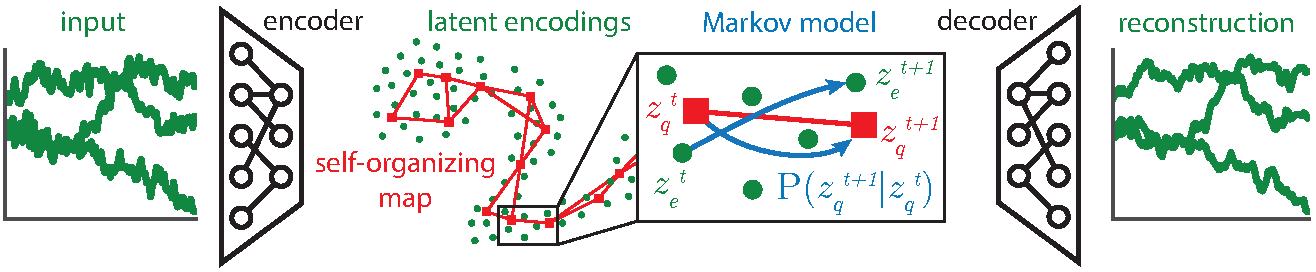
\includegraphics[width=\textwidth]{Overview_SOM-VAE.pdf}
    \caption{Schematic overview of our model architecture. Time series from the data space [green] are encoded by a neural network [black] time-point-wise into the latent space. The latent data manifold is approximated with a self-organizing map (SOM) [red]. In order to achieve a discrete representation, every latent data point ($z_e$) is mapped to its closest node in the SOM ($z_q$). A Markov transition model [blue] is learned to predict the next discrete representation ($z_q^{t+1}$) given the current one ($z_q^t$). The discrete representations can then be decoded by another neural network back into the original data space.}
    \label{fig:overview}
\end{figure}


A schematic overview of our proposed model is depicted in Figure \ref{fig:overview}.
An input $x \in \mathbb{R}^d$ is mapped to a latent encoding $z_e \in \mathbb{R}^m$ (usually $m < d$) by computing $z_e = f_{\theta}(x)$, where $f_{\theta}(\cdot)$ is parameterized by the encoder neural network.
The encoding is then assigned to an embedding $z_q \in \mathbb{R}^m$ in the dictionary of embeddings $E = \lbrace e_1, \dots, e_k \; \vert \; e_i \in \mathbb{R}^m \rbrace$ by sampling $z_q \sim p(z_q | z_e)$.
The form of this distribution is flexible and can be a design choice.
In order for the model to behave similarly to the original SOM algorithm (see below), in our experiments we choose the distribution to be categorical with probability mass 1 on the closest embedding to $z_e$, i.e.\ $p(z_q | z_e) = \mathds{1} \lbrack z_q = \argmin_{e \in E} \| z_e - e\|^2 \rbrack$, where $\mathds{1} \lbrack \cdot \rbrack$ is the indicator function.
A reconstruction $\hat{x}$ of the input can then be computed as $\hat{x} = g_{\phi}(z)$, where $g_{\phi}(\cdot)$ is parameterized by the decoder neural network.
Since the encodings and embeddings live in the same space, one can compute two different reconstructions, namely $\hat{x}_e = g_{\phi}(z_e)$ and $\hat{x}_q = g_{\phi}(z_q)$.

To achieve a topologically interpretable neighborhood structure, the embeddings are connected to form a self-organizing map.
A self-organizing map consists of $k$ nodes $V=\{v_1, \dots , v_k\}$, where every node corresponds to an embedding in the data space $e_v \in \mathbb{R}^d$ and a representation in a lower-dimensional discrete space $m_v \in M$, where usually $M \subset \mathbb{N}^2$.
During training on a data set $\mathcal{D} = \{x_1, \dots ,x_n\}$, a winner node $\tilde{v}$ is chosen for every point $x_i$ according to $\tilde{v} = \argmin_{v \in V} \| e_v - x_i \|^2$.
The embedding vector for every node $u \in V$ is then updated according to $e_u \leftarrow e_u + N(m_u,m_{\tilde{v}}) \eta (x_i - e_u)$, where $\eta$ is the learning rate and $N(m_u, m_{\tilde{v}})$ is a neighborhood function between the nodes defined on the representation space $M$.
There can be different design choices for $N(m_u, m_{\tilde{v}})$.
A more thorough review of the self-organizing map algorithm is deferred to the appendix (Sec.~\ref{sec:SOMs}).

We choose to use a two-dimensional SOM because it facilitates visualization similar to \citet{Tirunagari2015}.
Since we want the architecture to be trainable end-to-end, we cannot use the standard SOM training algorithm described above.
Instead, we devise a loss function term whose gradient corresponds to a weighted version of the original SOM update rule (see below).
We implement it in such a way that any time an embedding $e_{i,j}$ at position $(i,j)$ in the map gets updated, it also updates all the embeddings in its immediate neighborhood $N(e_{i,j})$.
The neighborhood is defined as $N(e_{i,j}) = \{ e_{i-1,j}, e_{i+1,j}, e_{i,j-1}, e_{i,j+1} \}$ for a two-dimensional map.

The loss function for a single input $x$ looks like
%
\begin{equation} \label{eq:L_somvae}
	\mathcal{L}_{\text{SOM-VAE}}(x, \hat{x}_q, \hat{x}_e) = \mathcal{L}_{\text{reconstruction}}(x, \hat{x}_q, \hat{x}_e) + \alpha \, \mathcal{L}_{\text{commitment}}(x) + \beta \, \mathcal{L}_{\text{SOM}}(x)
\end{equation}
%
where $x$, $z_e$, $z_q$, $\hat{x}_e$ and $\hat{x}_q$ are defined as above and $\alpha$ and $\beta$ are weighting hyperparameters.

Every term in this function is specifically designed to optimize a different model component.
The first term is the reconstruction loss $\mathcal{L}_{\text{reconstruction}}(x, \hat{x}_q, \hat{x}_e) = \| x - \hat{x}_q \|^2 + \| x - \hat{x}_e \|^2$.
The first subterm of this is the discrete reconstruction loss, which encourages the assigned SOM node $z_q(x)$ to be an informative representation of the input.
The second subterm encourages the encoding $z_e(x)$ to also be an informative representation.
This ensures that all parts of the model have a fully differentiable credit assignment path to the loss function, which facilitates training.
Note that the reconstruction loss corresponds to the evidence lower bound (ELBO) of the VAE part of our model \citep{Kingma2013}.
Since we assume a uniform prior over $z_q$, the KL-term in the ELBO is constant w.r.t.\ the parameters and can be ignored during optimization.

The term $\mathcal{L}_{\text{commitment}}$ encourages the encodings and assigned SOM nodes to be close to each other and is defined as $\mathcal{L}_{\text{commitment}}(x) = \| z_e(x) - z_q(x) \|^2$.
Closeness of encodings and embeddings should be expected to already follow from the $\mathcal{L}_{\text{reconstruction}}$ term in a fully differentiable architecture.
However, due to the non-differentiability of the embedding assignment in our model, the $\mathcal{L}_{\text{commitment}}$ term has to be explicitly added to the objective in order for the encoder to get gradient information about $z_q$.

The SOM loss $\mathcal{L}_{\text{SOM}}$ is defined as $\mathcal{L}_{\text{SOM}}(x) = \sum_{\tilde{e} \in N(z_q(x))} \| \tilde{e} - \text{sg}[z_e(x)] \|^2$, where $N(\cdot)$ is the set of neighbors in the discrete space as defined above and $\text{sg}[\cdot]$ is the gradient stopping operator that does not change the outputs during the forward pass, but sets the gradients to 0 during the backward pass.
It encourages the neighbors of the assigned SOM node $z_q$ to also be close to $z_e$, thus enabling the embeddings to exhibit a self-organizing map property, while stopping the gradients on $z_e$ such that the encoding is not pulled in the direction of the neighbors.
This term enforces a neighborhood relation between the discrete codes and encourages all SOM nodes to ultimately receive gradient information from the data.
The gradient stopping in this term is motivated by the observation that the data points themselves do not get moved in the direction of their assigned SOM node's neighbors in the original SOM algorithm either (see above).
We want to optimize the embeddings based on their neighbors, but not the respective encodings, since any single encoding should be as close as possible to its assigned embedding and not receive gradient information from any other embeddings that it is not assigned to.
Note that the gradient update of a specific SOM node in this formulation depends on its distance to the encoding, while the step size in the original SOM algorithm is constant.
It will be seen that this offers some benefits in terms of optimization and convergence (see Sec. \ref{sec:clustering_benchmark}).


\subsection{Overcoming the Non-Differentiability}\label{sec:non-differentiability}

The main challenge in optimizing our architecture is the non-differentiability of the discrete cluster assignment step.
Due to this, the gradients from the reconstruction loss cannot flow back into the encoder.
A model with a similar problem is the recently proposed vector-quantized VAE (VQ-VAE) \citep{Oord2017}.
It can be seen as being similar to a special case of our SOM-VAE model, where one sets $\beta = 0$, i.e. disables the SOM structure.

In order to mitigate the non-differentiability, the authors of the VQ-VAE propose to copy the gradients from $z_q$ to $z_e$.
They acknowledge that this is an \emph{ad hoc} approximation, but observed that it works well in their experiments.
Due to our smaller number of embeddings compared to the VQ-VAE setup, the average distance between an encoding and its closest embedding is much larger in our case.
The gradient copying (see above) thus ceases to be a feasible approximation, because the true gradients at points in the latent space which are farther apart will likely be very different.

In order to still overcome the non-differentiability issue, we propose to add the second reconstruction subterm to $\mathcal{L}_{\text{reconstruction}}$, where the reconstruction $\hat{x}_e$ is decoded directly from the encoding $z_e$.
This adds a fully differentiable credit assignment path from the loss to the encoder and encourages $z_e$ to also be an informative representation of the input, which is a desirable model feature.
Most importantly, it works well in practice (see Sec.\ \ref{sec:clustering_benchmark}).

Note that since $z_e$ is continuous and therefore much less constrained than $z_q$, this term is optimized easily and becomes small early in training.
After that, mostly the $z_q$-term contributes to $\mathcal{L}_{\text{reconstruction}}$.
One could therefore view the $z_e$-term as an initial encouragement to place the data encodings at sensible positions in the latent space, after which the actual clustering task dominates the training objective.



\subsection{Encouraging Smoothness over Time}\label{sec:probabilistic_model}

Our ultimate goal is to predict the development of time series in an interpretable way.
This means that not only the state representations should be interpretable, but so should be the prediction as well.
To this end, we use a temporal probabilistic model.

Learning a probabilistic model in a high-dimensional continuous space can be challenging.
Thus, we exploit the low-dimensional discrete space induced by our SOM to learn a temporal model.
For that, we define a system state as the assigned node in the SOM and then learn a Markov model for the transitions between those states.
The model is learned jointly with the SOM-VAE, where the loss function becomes
%
\begin{equation}\label{eq:L_prob}
    \mathcal{L}(x^{t-1}, x^t, \hat{x}_q^t, \hat{x}_e^t) = \mathcal{L}_{\text{SOM-VAE}}(x^t, \hat{x}_q^t, \hat{x}_e^t) + \gamma \, \mathcal{L}_{\text{transitions}}(x^{t-1}, x^t) + \tau \, \mathcal{L}_{\text{smoothness}}(x^{t-1}, x^t)
\end{equation}
%
with weighting hyperparameters $\gamma$ and $\tau$.

The term $\mathcal{L}_{\text{transitions}}$ encourages the probabilities of actually observed transitions to be high.
It is defined as $\mathcal{L}_{\text{transitions}}(x^{t-1}, x^t) = - \log P_{M} (z_q(x^{t-1}) \rightarrow z_q(x^t))$, with $P_{M} (z_q(x^{t-1}) \rightarrow z_q(x^t))$ being the probability of a transition from state $z_q(x^{t-1})$ to state $z_q(x^t)$ in the Markov model.

The term $\mathcal{L}_{\text{smoothness}}$ encourages the probabilities for transitions to nodes that are far away from the current data point to be low or respectively the nodes with high transition probabilities to be proximal.
It achieves this by taking large values only for transitions to far away nodes that have a high probability under the model.
It is defined as $\mathcal{L}_{\text{smoothness}}(x^{t-1}, x^t) = \mathbb{E}_{P_{M} \left( z_q(x^{t-1}) \rightarrow \tilde{e} \right) } \left[ \| \tilde{e} - z_e(x^t) \|^2 \right]$.
The probabilistic model can inform the evolution of the SOM through this term which encodes our prior belief that transitions in natural data happen smoothly and that future time points will therefore mostly be found in the neighborhood of previous ones.
In a setting where the data measurements are noisy, this improves the clustering by acting as a temporal smoother.



\section{Datasets}
\label{sec:dataset}

Since we evaluate meta-learned embeddings on two applications: speaker diarization and speaker verification, we use different corpora commonly used in evaluating these respective applications. We choose corpora obtained from both controlled and naturalisitc settings, with the former generally assumed relatively free from noise, reverberation and babble. We further choose additional corpora to assist with application-specific analysis of performance, such as the effect of domains and speaker characteristics (age) on diarization error rate (DER) and channel conditions on equal error rate (EER). A summary of the corpora used in this work is presented in Table~\ref{tab:corpora_overview}. Below, we provide details for each corpora.

\begin{table}[h]
\caption{Overview of training and evaluation corpora}
\label{tab:corpora_overview}
\centering{
\begin{tabular}{ccc} \\ \hline
\multicolumn{1}{c}{\multirow{2}{*}{\textbf{Training}}} & \multicolumn{2}{c}{\textbf{Evaluation}} \\ 
\multicolumn{1}{c}{} & Speaker Diarization & Speaker Verification \\ \hline
\rule{0pt}{2ex} Vox2 & AMI & Vox1 test \\
Vox1 dev & DIHARD II dev & VOiCES \\
 & ADOS-Mod3 & SITW \\ \hline
\end{tabular}}
\end{table}


\subsection{Voxceleb}
\label{subsec:data_vox}
The Voxceleb corpus \cite{chung2018Voxceleb2} consists of YouTube videos and audio of speech from celebrities with a balanced gender distribution. Over a million utterances from $\approx$7300 speakers are annotated with speaker labels. The utterances are collected from varied background conditions to simulate an in-the-wild collection. The Voxceleb corpus is further subdivided into Vox1 and Vox2 datasets. Following the baseline Kaldi recipe\footnote{https://github.com/kaldi-asr/kaldi/tree/master/egs/voxceleb/v2}, we use the dev and test splits from Vox2 and the dev split from Vox1 for embedding training. The test split from Vox1 is reserved for speaker verification. There exists no speaker overlap between the train set and Vox1-test set.

\subsection{VOICES}
The VOiCES corpora \cite{richey2018voices} was released as part of the VOiCES from a distance challenge\footnote{https://voices18.github.io/}. It consists of clean audio (Librispeech corpus\cite{panayotov_librispeech2015}) played inside multiple room configurations and recorded with microphones of different types and placed at different locations in the room. In addition, various distractor noise signals were played along with the source audio to simulate acoustically challenging conditions for speaker and speech recognition. Furthermore, the audio source was rotated in its position to simulate a real person. 
We use the evaluation portion of the corpus which is expected to contain more challenging room configurations \cite{evalplan_2019voices} than the development portion.
% Add stuff about near and far-field after you design the experiments

\subsection{SITW}
The speakers-in-the-wild corpus \cite{McLaren_SITWCorpus2016} was released as part of the SITW speaker recognition challenge. It consists of in-the-wild audio collected from a diverse range of recording and background conditions. In addition to speaker identities, the utterances are manually annotated for gender, extent of degradation, microphone type and other noise conditions in order to aid analysis. A subset of the utterances also include multiple speakers, with timing information available for the speaker with longest duration. 
A handful of speakers from the SITW corpus are known to overlap with the Voxceleb corpus~\footnote{\url{http://www.robots.ox.ac.uk/\~vgg/data/Voxceleb/SITW_overlap.txt}}. In this work, we remove the utterances corresponding to these speakers before evaluation. Details of corpora used in speaker verification is provided in Table~\ref{tab:spkrVerDataStats}.

\begin{table}[]
\caption{Statistics of corpora used for speaker verification, including trial subsets created for analysis purposes}
\label{tab:spkrVerDataStats}
\centering{
\begin{tabular}{llll} \\ \hline

\multicolumn{1}{c}{\textbf{Corpus}} & \multicolumn{1}{c}{\textbf{\#Spkrs}} & \multicolumn{1}{c}{\textbf{\#Utterances}} &
\textbf{\#Trails (\#target)} \\ \hline
%\multicolumn{1}{c}{\textbf{\begin{tabular}[c]{@{}c@{}}\#Trials\\ (\#target)\end{tabular}}} \\ \hline
% Vox1 test & 40 & 4715 & 37720 (18860/18860) \\
% VOiCES & 100 & 11392 & 3607516 (36443/3571073) \\
% VOiCES close mic & 98 & 1076 & 848001 (8523/839478)\\
% VOiCES far mic & 96 & 1006 & 778309 (7824/770485)\\
% VOiCES obs mic & 96 & 1006 & 777623 (7873/769750)\\
% SITW      & 151 & 1006 & 505506 (3034/502472)\\ 
% SITW low deg & 150 & 998 & 159796 (735/159061)\\
% SITW high deg & 151 & 1003 & 196358 (1264/195112)\\ \hline
Vox1 test & 40 & 4715 & 38K (19K) \\
VOiCES & 100 & 11392 & 3.6M (36K) \\
\quad close mic & 98 & 1076 & 0.84M (8.5K)\\
\quad far mic & 96 & 1006 & 0.78M (7.9K)\\
\quad obs mic & 96 & 1006 & 0.77M (7.9K)\\
SITW      & 151 & 1006 & 0.50M (3K)\\ 
\quad low deg & 150 & 998 & 0.16M (735)\\
\quad high deg & 151 & 1003 & 0.20M (1.2K)\\ \hline

\end{tabular}}
\end{table}

\subsection{AMI}
The AMI Meeting corpus\footnote{\url{http://groups.inf.ed.ac.uk/ami/corpus/}} consists of over 100 hours of office meetings recorded in four different locations. The meetings are recorded using both close-talk and far-field  microphones, we use the former for diarization purpose. Since each speaker has their individual channels, we beamformed the audio into a single channel. We follow \cite{sun_2019,moni_clusterGAN} for splitting the sessions into the dev and eval partitions, ensuring that no speakers overlap between them. For our purposes, the AMI sessions represent audio collected in noise-free recording conditions.

\subsection{DIHARD}
The DIHARD speaker diarization challenges \cite{ryant2018first} were introduced in order to focus on hard diarization tasks, i.e., in-the-wild data collected with naturalistic background conditions. In this work, we use the development set from second DIHARD challenge. This corpus consists of data from multiple domains such as clinical interviews, audiobooks, broadcast news, etc. We make use of the 192 sessions in the single-channel task in this work. It is worth noting that a handful of sessions in this corpus contain only a single speaker.

\begin{table}[h]
\caption{Statistics of corpora used for speaker diarization}
\label{tab:corpora_diar}
\begin{tabular}{ccccc} \\ \hline
Corpus & \#Sessions & \#Spkrs/Session & \multicolumn{1}{c}{\begin{tabular}[c]{@{}c@{}}Session Duration\\ (min: ($\mu \pm \sigma$))\end{tabular}} \\ \hline
%\multicolumn{1}{c}{\textbf{\begin{tabular}[c]{@{}c@{}}Session\\ Duration\end{tabular}}} \\ \hline
%Session Duration ($\mu, \sigma$)\\
DIHARD & 192 & 3.48 & 7.44 $\pm$ 3.00\\
AMI (dev+eval) & 26 & 3.96 & 31.54 $\pm$ 9.06\\
ADOS-Mod3& 173 & 2 & 3.23 $\pm$ 1.50 \\ \hline
\end{tabular}
\end{table}

\subsection{ADOS-Mod3}
\label{subsec:ados}
One of the most challenging domains from the DIHARD evaluations included speech collected from children. Speaker diarization for these interactions involve additional complexities due to two reasons: (1) An intrinsic variability in child speech owing to developmental factors \cite{Lee1999Acousticsofchildrensspeech:,lee2014developmental}, and (2) Speech abnormalities due to underlying neuro-developmental disorder such as autism. To this end, we use 173 child-adult interactions consisting of excerpts from the administration of module 3 of the ADOS (Autism Diagnosis Observation Module) \cite{Lord2000}. These interactions involve children with sufficiently developed linguistic skills, i,e., ability to form complete sentences. All the children in this study had a diagnosis of autism spectrum disorder (ASD) or attention deficit hyperactivity disorder (ADHD). The sessions were collected from two different locations and manually annotated using the SALT transcription guidelines\footnote{\url{https://www.saltsoftware.com/media/wysiwyg/tranaids/TranConvSummary.pdf}}. Details of corpora used for speaker diarization is provided in Table \ref{tab:corpora_diar}.





\section{Experiments}
We conduct experiments on two ultra-fine entity typing datasets, {\bf \textsc{UFET}} (English) and {\bf \textsc{CFET}} (Chinese). Their data statistics are shown in Table \ref{tab:stat}. We mainly focus on and report the macro-averaged recall at the recall and expand stage, and concern mainly on the macro-$F1$ of the final prediction at the filter stage. We also evaluate the {\bf \textsc{\name}} models on the fine-grained (130 types) and coarse-grained (9 types) settings of entity typing without the recall and expand stage.
\subsection{UFET and CFET}
\subsubsection{Recall Stage}
\label{sec:recall}
We compare the recall@$K$ on the test sets of {\bf \textsc{UFET}} and {\bf\textsc{CFET}} between the trained MLC model (introduced in \ref{sec:mlc}) and a traditional BM25 model \cite{bm25} in Figure \ref{fig:recall}. The MLC model uses the RoBERTa-large as backbone and is tuned based on the recall@$128$ on the development set. We use AdamW optimizer with a learning rate of $2\times10^{-5}$. Results show that MLC is a strong recall model, it consistently has better recall compared to BM25 on both {\bf\textsc{UFET}} and {\bf\textsc{CFET}} dataset, and the recall@$128$ reaches over $85\%$ on {\bf \textsc{UFET}}, and over $94\%$ on {\bf \textsc{CFET}}.

\begin{figure}[t]
     \centering
     \begin{subfigure}[h]{0.5\textwidth}
         \centering
         \includegraphics[width=\textwidth]{src/img/recall_compare_bm25.pdf}
         \label{fig:mb2}
     \end{subfigure}   
 \caption{Recall@$K$ of MLC and BM25.}
 \label{fig:recall}
\end{figure}

\subsection{Expand Stage}
\label{sec:expand}
In Table \ref{tab:expand}, we evaluate the F1 scores of all candidates expanded by exact match, and top-$10$ candidates expanded by the MLM using Bert-large. We also demonstrate the improvement of recall by using candidate expansion in Figure \ref{fig:expand_improvement}. On {\bf \textsc{UFET}} dataset, expanding around $32$ additional candidates based on $112$ MLC candidates results in $2\%$ higher recall compared to recalling all $128$ candidates by MLC. The recall of $128$ candidates after the expansion is comparable to the recall of $180$ candidates recalled from MLC. Similarly, expanding $10$ candidates is comparable to additionally recalling $80$ candidates using MLC.
In our experiments, we replace the last $48$ candidates recalled by MLC with the candidates recalled by MLM and Exact match for {\bf \textsc{UFET}} and $10$ for {\bf \textsc{CFET}}. We found the expand stage has a positive effect on the final performance of {\bf \textsc{\name}}s, and helps them reach SOTA performance (analyze in Sec. \ref{sec:analyze}).


\begin{table}[t]
\centering
\scalebox{0.75}{
\begin{tabular}{cccccc} 
\toprule
{\bf \textsc{Dataset}} & {\bf \textsc{Expand}} &   {\bf \textsc{P}}  & {\bf \textsc{R}}  &  {\bf \textsc{F1}} & \small{Avg \# Expanded}  \\ \midrule
\multirow{2}{*}{\bf \textsc{UFET}} & {\bf \textsc{Match}}      & 11.2   & 11.3     & 9.8    & 5.23     \\
      & {\bf \textsc{MLM}}  &  8.5     &   17.1   &  10.7  &    10    \\ \midrule
\multirow{2}{*}{\bf \textsc{CFET}} & {\bf \textsc{Match}}   &  11.4  &  14.5  & 11.2   & 4.57    \\
 & {\bf \textsc{MLM}}  & 21.3   &  19.5  & 17.7    & 10    \\ \midrule
\end{tabular}}
\caption{Evaluation of the recalled candidates.}
\label{tab:expand}
\end{table}
\begin{figure}[t]
     \centering
     \begin{subfigure}[h]{0.45\textwidth}
         \centering
         \includegraphics[width=\textwidth]{src/img/recall_ufet.pdf}
         \caption{Recall@$128$ on {\bf \textsc{UFET}} by including different number of expanded candidates. }
         \label{fig:c1}
     \end{subfigure}
     \vfill
     \begin{subfigure}[h]{0.45\textwidth}
         \centering
         \includegraphics[width=\textwidth]{src/img/recall_cfet.pdf}
         \caption{Recall@$64$ on {\bf \textsc{CFET}} by including different number of expanded candidates.}
         \label{fig:c2}
     \end{subfigure}
\caption{Demonstration of the effect of expand stage. $x$-axis represents the number of candidates expanded by MLM/MLM+MATCH among these $128$ candidates. }
\label{fig:expand_improvement}
\end{figure}
\label{sec:exp_expand}
\subsection{Filter Stage and Final Results.}
\begin{table}[h!]
\centering
\scalebox{0.73}{
\renewcommand{\arraystretch}{1}
\begin{tabular}{cllll} \toprule
\multicolumn{2}{l}{\bf \textit{Base Models on UFET} }     & \bf \textsc{P}    & \bf \textsc{R}   & \bf \textsc{F1}  \\ \midrule
\multicolumn{5}{l}{\emph{MLC-like models}}        \\
\color{blue} \bf \texttt{B}& {\bf \textsc{Box4Types}}\cite{box4types}  & 52.8 & 38.8 & 44.8  \\
\color{blue}\bf \texttt{B}& {\bf \textsc{LDET}}$^\dagger$  \cite{onoe-durrett-2019-learning}          & 51.5 & 33.0 & 40.1 \\ 
\color{blue}\bf \texttt{B}& {\bf \textsc{MLMET}}$^\dagger$   {\cite{mlmet}}   & 53.6 & 45.3 & 49.1  \\
\color{blue}\bf \texttt{B}& {\bf \textsc{PL}}  \cite{ding2021prompt}   & 57.8 & 40.7 & 47.7 \\
\color{blue}\bf \texttt{B}& {\bf \textsc{DFET}}    \cite{dfet}      & 55.6 & 44.7 & 49.5 \\
\color{blue}\bf \texttt{B}& {\bf \textsc{MLC}} (reimplemented by us) & 46.5 & 34.9 & 39.9 \\ 
\color{red}\bf \texttt{R}& {\bf \textsc{MLC}} (reimplemented by us) & 42.2 & 44.9 & 43.5 \\ \hline 
\multicolumn{5}{l}{\emph{Seq2seq based models}}      \\
\color{blue}\bf \texttt{B} & {\bf \textsc{LRN} }  {\cite{liu-etal-2021-fine}}              & 54.5 & 38.9 & 45.4  \\\hline
\multicolumn{5}{l}{\emph{Filter models under our recall-expand-filter paradigm}}      \\
\color{blue}\bf \texttt{B} & {\bf \textsc{Vanilla CE}$_{128}$}   & 47.2 & 48.5 & 47.8 \\ 
\color{blue}\bf \texttt{B} & {\bf \textsc{\name-S$_{128}$}} (Ours)  & 53.2 & 48.3 & {\bf 50.6} \\ 
\color{blue}\bf \texttt{B} & {\bf \textsc{\name-S$_{128}$ w/o C2C}}   (Ours)   & 52.3 & 48.3 & 50.2 \\ 
\color{blue}\bf \texttt{B} & {\bf \textsc{\name-B$_{128}$}} (Ours)    & 49.9 & 50.0 & 49.9 \\ 
\color{blue}\bf \texttt{B} & {\bf \textsc{\name-B$_{128}$ w/o C2C}} (Ours)     & 49.9 & 48.2 & 49.0 \\ \hline
\color{red}\bf \texttt{R} & {\bf \textsc{Vanilla CE}$_{128}$}   & 49.6 & 49.0 & 49.3 \\ 
\color{red}\bf \texttt{R} & {\bf \textsc{\name-S$_{128}$}} (Ours)  & 53.3 & 47.3 & 50.1 \\ 
\color{red}\bf \texttt{R} & {\bf \textsc{\name-S$_{128}$ w/o C2C}}   (Ours)  & 53.2 & 46.6 & 49.7 \\ 
\color{red}\bf \texttt{R} & {\bf \textsc{\name-B$_{128}$}} (Ours)  & 52.5 & 47.9 & 50.1 \\ 
\color{red}\bf \texttt{R} & {\bf \textsc{\name-B$_{128}$ w/o C2C}} (Ours)     & 52.7 & 46.4 & 49.3 \\ \hline
\midrule
\multicolumn{2}{l}{\bf \textit{Large Models on UFET} }     & \bf \textsc{P}    & \bf \textsc{R}   & \bf \textsc{F1}  \\ \midrule
\multicolumn{5}{l}{\emph{MLC-like models}}        \\
\color{red}\bf \texttt{R} & {\bf \textsc{MLC}}  \cite{npcrf}               & 47.8 & 40.4 & 43.8  \\
\color{red}\bf \texttt{R} & {\bf \textsc{MLC-NPCRF}} \cite{npcrf}             & 48.7 & 45.5 & 47.0  \\
\color{red}\bf \texttt{R} & {\bf \textsc{MLC-GCN}} \cite{xiong-etal-2019-imposing}     & 51.2 & 41.0 & 45.5 \\
\color{blue}\bf \texttt{B} & {\bf \textsc{PL}}  \cite{ding2021prompt}       & 59.3 & 42.6 & 49.6  \\
\color{blue}\bf \texttt{B} & {\bf \textsc{PL-NPCRF}}  \cite{npcrf}  & 55.3 & 46.7 & {50.6}\\ \hline
\multicolumn{4}{l}{\emph{Cross-encoder based models and {\bf \textsc{\name}}s}}      \\
\color{red}\bf \texttt{R} & {\bf \textsc{LITE+L}}  \cite{lite}             & 48.7 & 45.8 & 47.2  \\
\color{teal}\bf \texttt{RM} & {\bf \textsc{LITE+NLI+L}} \cite{lite} & 52.4 & 48.9 & {50.6} \\ \hline
\multicolumn{4}{l}{\emph{Filter models under our recall-expand-filter paradigm}}   \\ 
\color{blue}\bf \texttt{B} & {\bf \textsc{Vanilla CE$_{128}$}}   & 50.3 & 49.6 & 49.9 \\ 
\color{blue}\bf \texttt{B} & {\bf \textsc{\name-S$_{128}$}}  (Ours)   & 52.5 & 49.1 & 50.8 \\ 
\color{blue}\bf \texttt{B} & {\bf \textsc{\name-S$_{128}$ w/o C2C}}   (Ours)   & 54.1 & 47.1 & 50.4 \\ 
\color{blue}\bf \texttt{B} & {\bf \textsc{\name-B$_{128}$}} (Ours)    & 54.0 & 48.6 & 51.2 \\ 
\color{blue}\bf \texttt{B} & {\bf \textsc{\name-B$_{128}$ w/o C2C}} (Ours)     & 52.8 & 48.3 & 50.4 \\ \hline
\color{red}\bf \texttt{R} & {\bf \textsc{Vanilla CE$_{128}$}}   & 54.5 & 49.3 & 51.8 \\ 
\color{red}\bf \texttt{R} & {\bf \textsc{\name-S$_{128}$}}  (Ours)   & 50.8 & 49.8  &  50.3 \\ 
\color{red}\bf \texttt{R} & {\bf \textsc{\name-S$_{128}$ w/o C2C}}   (Ours)   & 51.5 & 48.8 & 50.1 \\ 
\color{red}\bf \texttt{R} & {\bf \textsc{\name-B$_{128}$}} (Ours)    & 51.9 & 50.8 & 51.4 \\ 
\color{red}\bf \texttt{R} & {\bf \textsc{\name-B$_{128}$ w/o C2C}} (Ours)     & 51.6 & 51.6 & 51.6 \\ \hline
\color{teal}\bf \texttt{RM} & {\bf \textsc{\name-B$_{128}$ w/o C2C}} (Ours) & 56.3 & 48.5 & {\bf 52.1} \\ \hline
\midrule
\end{tabular}}
\caption{Macro-averaged UFET result. {\bf \textsc{LITE+L}} is LITE without NLI pretraining, {\bf \textsc{LITE+L+NLI}} is the full LITE model. Methods marked by $\dagger$ utilize either distantly supervised or augmented data for training. {\bf \textsc{\name-S$_{128}$}} denotes we use $128$ candidates recalled and expanded from the first two stages.}
\label{tab:ufet}
\end{table}
\begin{table}[t]
\centering
\scalebox{0.75}{
\renewcommand{\arraystretch}{1}
\begin{tabular}{cllll} \toprule
\multicolumn{2}{l}{\bf \textit{Models on CFET} }     & \bf \textsc{P}    & \bf \textsc{R}   & \bf \textsc{F1}  \\ \midrule
\multicolumn{5}{l}{\emph{MLC-like models}}        \\
\color{purple}\bf \texttt{N}& {\bf \textsc{MLC}} & 55.8 & 58.6 & 57.1 \\  
\color{purple}\bf \texttt{N}& {\bf \textsc{MLC-NPCRF}} \cite{npcrf}     & 57.0 & 60.5 & 58.7 \\ 
\color{purple}\bf \texttt{N}& {\bf \textsc{MLC-GCN}} \cite{xiong-etal-2019-imposing}   & 51.6 & 63.2 & 56.8 \\ 
\color{brown}\bf \texttt{C}& {\bf \textsc{MLC}} & 54.0 & 59.5 & 56.6 \\  
\color{brown}\bf \texttt{C}& {\bf \textsc{MLC-NPCRF}} \cite{npcrf}   & 54.0 & 61.6 & 57.3 \\  
\color{brown}\bf \texttt{C}& {\bf \textsc{MLC-GCN}} \cite{xiong-etal-2019-imposing} & 56.4 & 58.6 & 57.5 \\ \midrule 
\multicolumn{5}{l}{\emph{Filter models under our recall-expand-filter paradigm}}      \\
\color{purple}\bf \texttt{N} & {\bf \textsc{Vanilla CE}}   & 57.6 & 64.3 & 60.7 \\ 
\color{brown}\bf \texttt{C} & {\bf \textsc{Vanilla CE}}   & 54.0 & 63.3 & 58.3 \\  \hline
\color{purple}\bf \texttt{N} & {\bf \textsc{\name-S$_{64}$}} (Ours)  & 58.4 & 62.1 & 60.2 \\ 
\color{purple}\bf \texttt{N} & {\bf \textsc{\name-S$_{64}$ w/o C2C}}   (Ours)   & 59.1 & 61.5 & 60.3 \\ 
\color{purple}\bf \texttt{N} & {\bf \textsc{\name-B$_{64}$}} (Ours)    & 56.7 & 66.1 & 61.1 \\ 
\color{purple}\bf \texttt{N} & {\bf \textsc{\name-B$_{64}$ w/o C2C}} (Ours)     & 58.8 & 64.1 & 61.4 \\ \hline
\color{brown}\bf \texttt{C} & {\bf \textsc{\name-S$_{64}$}} (Ours)  & 55.5 & 62.6 & 58.8 \\ 
\color{brown}\bf \texttt{C} & {\bf \textsc{\name-S$_{64}$ w/o C2C}}   (Ours)   & 54.0 & 63.4 & 58.3 \\ 
\color{brown}\bf \texttt{C} & {\bf \textsc{\name-B$_{64}$}} (Ours)    & 55.0 & 63.5 & 59.0 \\ 
\color{brown}\bf \texttt{C} & {\bf \textsc{\name-B$_{64}$ w/o C2C}} (Ours)     & 57.3 & 61.3 & 59.3 \\ \hline
\midrule
\end{tabular}}
\caption{Macro-averaged CFET result.}
\label{tab:cfet}
\end{table}

In this section, we report the performance of {\bf \textsc{MCCE}} variants as the filter models and compare them with various strong baselines that we will introduce later. We also compare the inference speed of different models in this section. For filter models, we treat the number of candidates $K$ recalled and expanded by the first two stages as hyper-parameters, and tune it on the development set. We found the choice of PLM backbones has a non-negligible effect on the performance, and the PLM backbone of previous methods varies. Therefore for fairer comparisons to baselines, we conduct experiments of {\bf \textsc{\name}} using different backbone PLMs for our {\bf \textsc{\name}} models and report the results. For all {\bf \textsc{\name}} models, we use AdamW optimizer with a learning rate tuned between $5\times 10^{-6}$ and $2\times 10^{-5}$. The batch size we use is $4$ and we train the models for at most $50$ epochs with early stopping. {\bf \textsc{UFET}} also provides a large dataset obtained from distant supervision such as entity linking, we do not use it and only train and evaluate our models on human-labeled data.
\paragraph{Baselines}
The {\bf \textsc{MLC}} model we used for the recall stage and the cross-encoder ({\bf \textsc{CE}}) we introduced in Sec. \ref{sec:vanilla_ce} are natural baselines. We also compare our methods with recent PLM-based methods. {\bf \textsc{LDET} }\cite{onoe-durrett-2019-learning} is an MLC with Bert-base-uncased and ELMo \cite{elmo} trained on 727k examples automatically denoised from the distantly labeled UFET. {\bf \textsc{GCN} }\cite{xiong-etal-2019-imposing} uses GCN to model type correlations and obtain type embeddings. Types are scored by dot-product of mention and type embeddings. The original paper uses BiLSTM as the mention encoder and we use the results re-implemented by \citet{npcrf} using RoBERTa-large. {\bf \textsc{Box4Type} }\cite{box4types} uses Bert-large as the backbone and uses box embedding to encode mentions and types for training and inference. {\bf \textsc{LRN} }\cite{liu-etal-2021-fine} use Bert-base as the encoder and an LSTM decoder to generate types in a seq2seq manner. {\bf \textsc{MLMET} }\cite{mlmet} is a {\bf \textsc{MLC}} with Bert-base, but first pretrained by the distantly-labeled data augmented by masked word prediction, then finetuned and self-trained on the 2k human-annotated data. {\bf \textsc{PL}} \cite{ding2021prompt} uses prompt learning for entity typing. {\bf \textsc{DFET} }\cite{dfet} uses {\bf \textsc{PL}} as backbone and is a multi-round automatic denoising method for 2k labeled data. {\bf \textsc{LITE} }\cite{lite} is the previous SOTA system that formulates entity typing as textual inference. {\bf \textsc{LITE}} uses RoBERTa-large-MNLI as the backbone, and is a cross-encoder (introduced in Sec. \ref{sec:vanilla_ce}) with designed templates and a hierarchical loss. \citet{npcrf} proposes {\bf \textsc{NPCRF}} to enhance backbones such as {\bf \textsc{PL}} and {\bf \textsc{MLC}} by modeling type correlations, and reach performance comparable to {\bf \textsc{LITE}}.

\paragraph{Naming Conventions}
Let {\bf \textsc{\name-S}} be the {\bf \textsc{\name}} model that treats candidates as sub-tokens, and {\bf \textsc{\name-B}} be the model representing candidates as fixed-size blocks. The {\bf \textsc{\name}} model without {\bf \textsc{C2C}} attention (mentioned in Sec. \ref{sec:attn}) is denoted as {\bf \textsc{\name-B} w/o C2C}. For PLM backbones used in {\bf \textsc{UFET}}, we use {\color{blue} \bf \texttt{B}}, {\color{red} \bf \texttt{R}}, {\color{teal} \bf \texttt{RM}} to denote BERT-base-cased \cite{bert}, RoBERTa \cite{liu2019roberta}, and RoBERTa-MNLI \cite{liu2019roberta} respectively. For {\bf \textsc{CFET}}, we adopt two widely-used Chinese PLM, BERT-base-Chinese and NeZha-base-Chinese, and denote them as {\color{brown} \bf \texttt{C}} and {\color{purple} \bf \texttt{N}} respectively. 

\paragraph{UFET Results} We show the results of {\bf \textsc{UFET}} dataset in Table \ref{tab:ufet}. The results show that: (1) The recall-expand-filter paradigm is effective. Filter models outperform all baselines without the paradigm by a large margin. The vanilla CE under our paradigm reaches $51.8$ F1 compared to more complexed CE {\bf \textsc{LITE}} with $50.6$ F1 (2) {\bf \textsc{\name}} models reach SOTA performances. {\bf \textsc{\name-S$_{128}$}} with BERT-base performs best and reaches {\bf 50.6} F1 score, which is comparable to previous SOTA performance of large models such as {\bf \textsc{LITE+NLI+L}} and {\bf \textsc{PL+NPCRF}}. Among large models, {\bf \textsc{\name-B$_{128}$ w/o C2C}} also reaches SOTA performance with {\bf 52.1} F1 score. (3) {\bf \textsc{C2C}} attention is not necessary on large models, but is useful in base models. (4) Large models can utilize type semantics better. We found {\bf \textsc{\name-B}} outperforms {\bf \textsc{\name-S}} on large models, but underperforms {\bf \textsc{\name-S}} on base models. (5) Backbone PLM matters. We found the performance of {\bf \textsc{Vannila CE}} under our paradigm is largely affected by the PLM it used. It reaches $47.8$ F1 with BERT-base and $51.8$ F1 with RoBERTa-large. For {\bf \textsc{\name}} models, we found {\bf \textsc{\name}} performs better than {\bf \textsc{\name-B}} with BERT, and worse than {\bf \textsc{\name-B}} with RoBERTa. 

\begin{table*}[t]
\centering
\scalebox{0.9}{
\begin{tabular}{lllcc} \toprule
\bf \textsc{Model}  & \bf \textsc{\# FP} & \bf \textsc{Attn} & \bf \textsc{sents/sec} & \bf \textsc{F1} \\ \midrule
{\bf \textsc{MLC}} & \small{$1$}  & \small{$L_S^2D$} & 58.8 & 43.8\\
{\bf \textsc{LITE+NLI+L (CE)}}  & \small{$N$}  & \small{$L_S^2D$} & 0.02 & 50.6\\ \midrule \hline
\multicolumn{5}{l}{\emph{filter stage inference speed.}}  \\
{\bf \textsc{Vanilla CE$_{128}$}}  & \small{$128$}  & \small{$L_S^2D$} & 1.64 & 51.8 \\ 
{\bf \textsc{\name-S$_{128}$}}  & \small{$1$}  & \small{$(L_S+128)^2D$} & 60.8 & 50.1 \\ 
{\bf \textsc{\name-B$_{128}$}}  & \small{$1$}  & \small{$(L_S+128B)^2D$} & 22.3 & 51.4\\ 
{\bf \textsc{\name-B$_{128}$ w/o C2C}}  & \small{$1$}  & \small{$(L_S^2+256L_S B + 128 B^2)D$} & 25.2 & {\bf 52.1}\\ \bottomrule
\end{tabular}}
\caption{Inference speed comparison of models. {\bf \textsc{\# FP}} means the number of PLM forward passes required by a single inference. {\bf \textsc{ATTN}} column lists the theoretical attention complexity.  We also report the practical inference speed {\bf \textsc{sents/sec}} and the {\bf \textsc{F1}} scores on {\bf \textsc{UFET}} with RoBERTa-large architecture.}
\label{tab:speed}
\end{table*}

\begin{table}[t]
\centering
\scalebox{0.85}{
\renewcommand{\arraystretch}{1}
\begin{tabular}{cllll} \toprule
\multicolumn{2}{l}{\bf \textit{Models} }     & \bf \textsc{P}    & \bf \textsc{R}   & \bf \textsc{F1}  \\ \midrule
\multicolumn{5}{l}{\emph{coarse (9 types) Open Entity}}        \\ \hline
\color{red}\bf \texttt{R} & {\bf \textsc{MLC}}   & 76.8 & 78.5 & 77.6 \\ 
\color{red}\bf \texttt{R} & {\bf \textsc{Vanilla CE$_{9}$}}   & 82.3 & 81.0 & 81.6 \\ 
\color{red}\bf \texttt{R} & {\bf \textsc{\name-S$_{9}$}}   & 77.0 & 87.7 & 82.0 \\ 
\color{red}\bf \texttt{R} & {\bf \textsc{\name-B$_{9}$ w/o C2C}}   & 77.2 & 85.4 & 81.1 \\ \hline
\multicolumn{5}{l}{\emph{fine (130 types)}}        \\ \hline
\color{red}\bf \texttt{R} & {\bf \textsc{MLC}}   & 70.4 & 63.7 & 66.9  \\ 
\color{red}\bf \texttt{R} & {\bf \textsc{Vanilla CE}$_{130}$}   & 67.9 & 66.4 & 67.1 \\ 
\color{red}\bf \texttt{R} & {\bf \textsc{\name-S$_{130}$}}   & 65.8 & 71.8 & 68.7 \\ 
\color{red}\bf \texttt{R} & {\bf \textsc{\name-B$_{130}$ w/o C2C}}   & 64.1 & 70.5 & 67.1 \\ \hline
\midrule
\end{tabular}}
\caption{Micro-averaged results on UFET fine and coarse.}
\label{tab:ufet-coarse-fine}
\end{table}

\paragraph{CFET Results} We conduct experiments on {\bf \textsc{CFET}} and compare {\bf \textsc{\name}} models with several strong baselines:  {\bf \textsc{NPCRF}} and {\bf \textsc{GCN}} with MLC-like architecture, and {\bf \textsc{Vanilla CE}} under out paradigm which is proved to be better than {\bf \textsc{LITE}} on {\bf \textsc{UFET}}. The results are shown in Table \ref{tab:cfet}. Similar to results in {\bf \textsc{UFET}}, filter models under our paradigm significantly outperform MLC-like baselines, $+2.0$ F1 for Nezha-base and $+1.8$ F1 for BERT-base-Chinese. In {\bf \textsc{CFET}}, {\bf \textsc{\name}-B} is significantly better than {\bf \textsc{\name}-S}, on both Nezha-base and BERT-base-Chinese, indicating the importance of type semantics in Chinese language. We also find that {\bf \textsc{\name} w/o C2C} is generally better than  {\bf \textsc{\name} w/ C2C}, it is possibly because the C2C attention distracts the candidates from attending to mention and contexts.
\paragraph{Speed Comparison} Table \ref{tab:speed} shows the theoretical inference complexity (number of PLM forward passes, and attention complexity), and practical inference speed (number of sentences inferred per second) of different models. We conduct the speed test using NVIDIA TITAN RTX for all models, and the inference batch size is 4.
At the filter stage, the inference speed of {\bf \textsc{\name-S}} is on par with {\bf \textsc{MLC}} (even slightly faster because we don't need to score all types), and is about 40 times faster than {\bf \textsc{Vannila CE}} and thousands of times faster than {\bf \textsc{LITE}}. {\bf \textsc{\name-B w/o C2C}} is not significantly faster than {\bf \textsc{\name-B}} as expected. It's possibly because the computation related to the block attention is not fully optimized by existing deep learning frameworks. The speed advantage of {\bf \textsc{\name-B w/o C2C}} over {\bf \textsc{\name-B}} will be greater with more candidates.


\subsection{Fine-grained and Coarse-grained Entity Typing}
We also conduct experiments on Fine-grained (130-class) and Coarse-grained (9-class, also known as ``Open Entity'') entity typing, and the results are shown in Table \ref{tab:ufet-coarse-fine}. As the type candidate set is much smaller in these settings, we skip the recall and expand stages and directly run the filter models and compare them to baselines. Results show that both {\bf \textsc{\name}-S} and {\bf \textsc{\name}-B} are still better than {\bf \textsc{MLC}} and {\bf \textsc{Vanilla CE}}, and {\bf \textsc{\name}-S} is better than {\bf \textsc{\name}-B} on coarser-grained cases possibly because the coarser-grained types are simpler in surface-forms and {\bf \textsc{\name}-S} will not lose many type semantics.






\section{Conclusion}
\label{ss: conclusion}

% summary of approach
This paper presents a methodology to evaluate the effectiveness of evasions and its application to studying PDF malware scanners.
Our implementation of the methodology, the Chameleon framework, automatically generates and enriches malicious documents with one or multiple evasions.
We use these documents for an in-depth study of \nbAnalyzers{} PDF scanners and how they are affected by evasions.
More broadly, our methodology can also be used for studying evasions of other malware types, e.g., malicious executables.

% main take-aways
The overall result of our study is cause for concern.
We show that the studied evasions are surprisingly effective in fooling state-of-the-art scanners.
In particular by combining evasions, attackers can bypass modern defenses in both static and dynamic scanners.
Moreover, we find huge variations across scanners, enabling targeted attacks based on evasions picked specifically for a targeted scanner.
All these findings are a call to arms for future work on anti-evasion techniques.

Our work will support future efforts toward improving malware scanners in several ways.
First, the results of our study help security vendors to better understand their vulnerability to specific evasions and to focus their attention on mitigating the most effective evasions.
Second, we are releasing the corpus of malicious, evasive documents generated by Chameleon as a ready-to-use benchmark.
We are in contact with several developers of PDF scanners, and some of them, e.g., SploitGuard and SAFE-PDF, have already used our benchmark to test and improve their security scanners.
Finally, the Chameleon framework provides a basis for expanding the set of benchmarks by incorporating future evasions, exploits, and payloads.


% % use section* for acknowledgment
% \section*{Acknowledgment}
% The authors would like to thank...

% references section

\bibliographystyle{IEEEtran}
\bibliography{mybib}

% Instructions for photo, bibliography, etc available in bare_jrnl.tex


% that's all folks
\end{document}




%% bare_jrnl.tex
%% V1.4b
%% 2015/08/26
%% by Michael Shell
%% see http://www.michaelshell.org/
%% for current contact information.
%%
%% This is a skeleton file demonstrating the use of IEEEtran.cls
%% (requires IEEEtran.cls version 1.8b or later) with an IEEE
%% journal paper.
%%
%% Support sites:
%% http://www.michaelshell.org/tex/ieeetran/
%% http://www.ctan.org/pkg/ieeetran
%% and
%% http://www.ieee.org/

%%*************************************************************************
%% Legal Notice:
%% This code is offered as-is without any warranty either expressed or
%% implied; without even the implied warranty of MERCHANTABILITY or
%% FITNESS FOR A PARTICULAR PURPOSE! 
%% User assumes all risk.
%% In no event shall the IEEE or any contributor to this code be liable for
%% any damages or losses, including, but not limited to, incidental,
%% consequential, or any other damages, resulting from the use or misuse
%% of any information contained here.
%%
%% All comments are the opinions of their respective authors and are not
%% necessarily endorsed by the IEEE.
%%
%% This work is distributed under the LaTeX Project Public License (LPPL)
%% ( http://www.latex-project.org/ ) version 1.3, and may be freely used,
%% distributed and modified. A copy of the LPPL, version 1.3, is included
%% in the base LaTeX documentation of all distributions of LaTeX released
%% 2003/12/01 or later.
%% Retain all contribution notices and credits.
%% ** Modified files should be clearly indicated as such, including  **
%% ** renaming them and changing author support contact information. **
%%*************************************************************************


% *** Authors should verify (and, if needed, correct) their LaTeX system  ***
% *** with the testflow diagnostic prior to trusting their LaTeX platform ***
% *** with production work. The IEEE's font choices and paper sizes can   ***
% *** trigger bugs that do not appear when using other class files.       ***                          ***
% The testflow support page is at:
% http://www.michaelshell.org/tex/testflow/



\documentclass[journal]{IEEEtran}
%
% If IEEEtran.cls has not been installed into the LaTeX system files,
% manually specify the path to it like:
% \documentclass[journal]{../sty/IEEEtran}





% Some very useful LaTeX packages include:
% (uncomment the ones you want to load)


% *** MISC UTILITY PACKAGES ***
%
%\usepackage{ifpdf}
% Heiko Oberdiek's ifpdf.sty is very useful if you need conditional
% compilation based on whether the output is pdf or dvi.
% usage:
% \ifpdf
%   % pdf code
% \else
%   % dvi code
% \fi
% The latest version of ifpdf.sty can be obtained from:
% http://www.ctan.org/pkg/ifpdf
% Also, note that IEEEtran.cls V1.7 and later provides a builtin
% \ifCLASSINFOpdf conditional that works the same way.
% When switching from latex to pdflatex and vice-versa, the compiler may
% have to be run twice to clear warning/error messages.






% *** CITATION PACKAGES ***
%
%\usepackage{cite}
% cite.sty was written by Donald Arseneau
% V1.6 and later of IEEEtran pre-defines the format of the cite.sty package
% \cite{} output to follow that of the IEEE. Loading the cite package will
% result in citation numbers being automatically sorted and properly
% "compressed/ranged". e.g., [1], [9], [2], [7], [5], [6] without using
% cite.sty will become [1], [2], [5]--[7], [9] using cite.sty. cite.sty's
% \cite will automatically add leading space, if needed. Use cite.sty's
% noadjust option (cite.sty V3.8 and later) if you want to turn this off
% such as if a citation ever needs to be enclosed in parenthesis.
% cite.sty is already installed on most LaTeX systems. Be sure and use
% version 5.0 (2009-03-20) and later if using hyperref.sty.
% The latest version can be obtained at:
% http://www.ctan.org/pkg/cite
% The documentation is contained in the cite.sty file itself.






% *** GRAPHICS RELATED PACKAGES ***
%
\ifCLASSINFOpdf
  % \usepackage[pdftex]{graphicx}
  % declare the path(s) where your graphic files are
  % \graphicspath{{../pdf/}{../jpeg/}}
  % and their extensions so you won't have to specify these with
  % every instance of \includegraphics
  % \DeclareGraphicsExtensions{.pdf,.jpeg,.png}
\else
  % or other class option (dvipsone, dvipdf, if not using dvips). graphicx
  % will default to the driver specified in the system graphics.cfg if no
  % driver is specified.
  % \usepackage[dvips]{graphicx}
  % declare the path(s) where your graphic files are
  % \graphicspath{{../eps/}}
  % and their extensions so you won't have to specify these with
  % every instance of \includegraphics
  % \DeclareGraphicsExtensions{.eps}
\fi
% graphicx was written by David Carlisle and Sebastian Rahtz. It is
% required if you want graphics, photos, etc. graphicx.sty is already
% installed on most LaTeX systems. The latest version and documentation
% can be obtained at: 
% http://www.ctan.org/pkg/graphicx
% Another good source of documentation is "Using Imported Graphics in
% LaTeX2e" by Keith Reckdahl which can be found at:
% http://www.ctan.org/pkg/epslatex
%
% latex, and pdflatex in dvi mode, support graphics in encapsulated
% postscript (.eps) format. pdflatex in pdf mode supports graphics
% in .pdf, .jpeg, .png and .mps (metapost) formats. Users should ensure
% that all non-photo figures use a vector format (.eps, .pdf, .mps) and
% not a bitmapped formats (.jpeg, .png). The IEEE frowns on bitmapped formats
% which can result in "jaggedy"/blurry rendering of lines and letters as
% well as large increases in file sizes.
%
% You can find documentation about the pdfTeX application at:
% http://www.tug.org/applications/pdftex





% *** MATH PACKAGES ***
%
%\usepackage{amsmath}
% A popular package from the American Mathematical Society that provides
% many useful and powerful commands for dealing with mathematics.
%
% Note that the amsmath package sets \interdisplaylinepenalty to 10000
% thus preventing page breaks from occurring within multiline equations. Use:
%\interdisplaylinepenalty=2500
% after loading amsmath to restore such page breaks as IEEEtran.cls normally
% does. amsmath.sty is already installed on most LaTeX systems. The latest
% version and documentation can be obtained at:
% http://www.ctan.org/pkg/amsmath





% *** SPECIALIZED LIST PACKAGES ***
%
%\usepackage{algorithmic}
% algorithmic.sty was written by Peter Williams and Rogerio Brito.
% This package provides an algorithmic environment fo describing algorithms.
% You can use the algorithmic environment in-text or within a figure
% environment to provide for a floating algorithm. Do NOT use the algorithm
% floating environment provided by algorithm.sty (by the same authors) or
% algorithm2e.sty (by Christophe Fiorio) as the IEEE does not use dedicated
% algorithm float types and packages that provide these will not provide
% correct IEEE style captions. The latest version and documentation of
% algorithmic.sty can be obtained at:
% http://www.ctan.org/pkg/algorithms
% Also of interest may be the (relatively newer and more customizable)
% algorithmicx.sty package by Szasz Janos:
% http://www.ctan.org/pkg/algorithmicx




% *** ALIGNMENT PACKAGES ***
%
%\usepackage{array}
% Frank Mittelbach's and David Carlisle's array.sty patches and improves
% the standard LaTeX2e array and tabular environments to provide better
% appearance and additional user controls. As the default LaTeX2e table
% generation code is lacking to the point of almost being broken with
% respect to the quality of the end results, all users are strongly
% advised to use an enhanced (at the very least that provided by array.sty)
% set of table tools. array.sty is already installed on most systems. The
% latest version and documentation can be obtained at:
% http://www.ctan.org/pkg/array


% IEEEtran contains the IEEEeqnarray family of commands that can be used to
% generate multiline equations as well as matrices, tables, etc., of high
% quality.




% *** SUBFIGURE PACKAGES ***
%\ifCLASSOPTIONcompsoc
%  \usepackage[caption=false,font=normalsize,labelfont=sf,textfont=sf]{subfig}
%\else
%  \usepackage[caption=false,font=footnotesize]{subfig}
%\fi
% subfig.sty, written by Steven Douglas Cochran, is the modern replacement
% for subfigure.sty, the latter of which is no longer maintained and is
% incompatible with some LaTeX packages including fixltx2e. However,
% subfig.sty requires and automatically loads Axel Sommerfeldt's caption.sty
% which will override IEEEtran.cls' handling of captions and this will result
% in non-IEEE style figure/table captions. To prevent this problem, be sure
% and invoke subfig.sty's "caption=false" package option (available since
% subfig.sty version 1.3, 2005/06/28) as this is will preserve IEEEtran.cls
% handling of captions.
% Note that the Computer Society format requires a larger sans serif font
% than the serif footnote size font used in traditional IEEE formatting
% and thus the need to invoke different subfig.sty package options depending
% on whether compsoc mode has been enabled.
%
% The latest version and documentation of subfig.sty can be obtained at:
% http://www.ctan.org/pkg/subfig




% *** FLOAT PACKAGES ***
%
%\usepackage{fixltx2e}
% fixltx2e, the successor to the earlier fix2col.sty, was written by
% Frank Mittelbach and David Carlisle. This package corrects a few problems
% in the LaTeX2e kernel, the most notable of which is that in current
% LaTeX2e releases, the ordering of single and double column floats is not
% guaranteed to be preserved. Thus, an unpatched LaTeX2e can allow a
% single column figure to be placed prior to an earlier double column
% figure.
% Be aware that LaTeX2e kernels dated 2015 and later have fixltx2e.sty's
% corrections already built into the system in which case a warning will
% be issued if an attempt is made to load fixltx2e.sty as it is no longer
% needed.
% The latest version and documentation can be found at:
% http://www.ctan.org/pkg/fixltx2e


%\usepackage{stfloats}
% stfloats.sty was written by Sigitas Tolusis. This package gives LaTeX2e
% the ability to do double column floats at the bottom of the page as well
% as the top. (e.g., "\begin{figure*}[!b]" is not normally possible in
% LaTeX2e). It also provides a command:
%\fnbelowfloat
% to enable the placement of footnotes below bottom floats (the standard
% LaTeX2e kernel puts them above bottom floats). This is an invasive package
% which rewrites many portions of the LaTeX2e float routines. It may not work
% with other packages that modify the LaTeX2e float routines. The latest
% version and documentation can be obtained at:
% http://www.ctan.org/pkg/stfloats
% Do not use the stfloats baselinefloat ability as the IEEE does not allow
% \baselineskip to stretch. Authors submitting work to the IEEE should note
% that the IEEE rarely uses double column equations and that authors should try
% to avoid such use. Do not be tempted to use the cuted.sty or midfloat.sty
% packages (also by Sigitas Tolusis) as the IEEE does not format its papers in
% such ways.
% Do not attempt to use stfloats with fixltx2e as they are incompatible.
% Instead, use Morten Hogholm'a dblfloatfix which combines the features
% of both fixltx2e and stfloats:
%
% \usepackage{dblfloatfix}
% The latest version can be found at:
% http://www.ctan.org/pkg/dblfloatfix




%\ifCLASSOPTIONcaptionsoff
%  \usepackage[nomarkers]{endfloat}
% \let\MYoriglatexcaption\caption
% \renewcommand{\caption}[2][\relax]{\MYoriglatexcaption[#2]{#2}}
%\fi
% endfloat.sty was written by James Darrell McCauley, Jeff Goldberg and 
% Axel Sommerfeldt. This package may be useful when used in conjunction with 
% IEEEtran.cls'  captionsoff option. Some IEEE journals/societies require that
% submissions have lists of figures/tables at the end of the paper and that
% figures/tables without any captions are placed on a page by themselves at
% the end of the document. If needed, the draftcls IEEEtran class option or
% \CLASSINPUTbaselinestretch interface can be used to increase the line
% spacing as well. Be sure and use the nomarkers option of endfloat to
% prevent endfloat from "marking" where the figures would have been placed
% in the text. The two hack lines of code above are a slight modification of
% that suggested by in the endfloat docs (section 8.4.1) to ensure that
% the full captions always appear in the list of figures/tables - even if
% the user used the short optional argument of \caption[]{}.
% IEEE papers do not typically make use of \caption[]'s optional argument,
% so this should not be an issue. A similar trick can be used to disable
% captions of packages such as subfig.sty that lack options to turn off
% the subcaptions:
% For subfig.sty:
% \let\MYorigsubfloat\subfloat
% \renewcommand{\subfloat}[2][\relax]{\MYorigsubfloat[]{#2}}
% However, the above trick will not work if both optional arguments of
% the \subfloat command are used. Furthermore, there needs to be a
% description of each subfigure *somewhere* and endfloat does not add
% subfigure captions to its list of figures. Thus, the best approach is to
% avoid the use of subfigure captions (many IEEE journals avoid them anyway)
% and instead reference/explain all the subfigures within the main caption.
% The latest version of endfloat.sty and its documentation can obtained at:
% http://www.ctan.org/pkg/endfloat
%
% The IEEEtran \ifCLASSOPTIONcaptionsoff conditional can also be used
% later in the document, say, to conditionally put the References on a 
% page by themselves.




% *** PDF, URL AND HYPERLINK PACKAGES ***
%
%\usepackage{url}
% url.sty was written by Donald Arseneau. It provides better support for
% handling and breaking URLs. url.sty is already installed on most LaTeX
% systems. The latest version and documentation can be obtained at:
% http://www.ctan.org/pkg/url
% Basically, \url{my_url_here}.




% *** Do not adjust lengths that control margins, column widths, etc. ***
% *** Do not use packages that alter fonts (such as pslatex).         ***
% There should be no need to do such things with IEEEtran.cls V1.6 and later.
% (Unless specifically asked to do so by the journal or conference you plan
% to submit to, of course. )


% correct bad hyphenation here
\hyphenation{op-tical net-works semi-conduc-tor}


\begin{document}
%
% paper title
% Titles are generally capitalized except for words such as a, an, and, as,
% at, but, by, for, in, nor, of, on, or, the, to and up, which are usually
% not capitalized unless they are the first or last word of the title.
% Linebreaks \\ can be used within to get better formatting as desired.
% Do not put math or special symbols in the title.
\title{Bare Demo of IEEEtran.cls\\ for IEEE Journals}
%
%
% author names and IEEE memberships
% note positions of commas and nonbreaking spaces ( ~ ) LaTeX will not break
% a structure at a ~ so this keeps an author's name from being broken across
% two lines.
% use \thanks{} to gain access to the first footnote area
% a separate \thanks must be used for each paragraph as LaTeX2e's \thanks
% was not built to handle multiple paragraphs
%

\author{Michael~Shell,~\IEEEmembership{Member,~IEEE,}
        John~Doe,~\IEEEmembership{Fellow,~OSA,}
        and~Jane~Doe,~\IEEEmembership{Life~Fellow,~IEEE}% <-this % stops a space
\thanks{M. Shell was with the Department
of Electrical and Computer Engineering, Georgia Institute of Technology, Atlanta,
GA, 30332 USA e-mail: (see http://www.michaelshell.org/contact.html).}% <-this % stops a space
\thanks{J. Doe and J. Doe are with Anonymous University.}% <-this % stops a space
\thanks{Manuscript received April 19, 2005; revised August 26, 2015.}}

% note the % following the last \IEEEmembership and also \thanks - 
% these prevent an unwanted space from occurring between the last author name
% and the end of the author line. i.e., if you had this:
% 
% \author{....lastname \thanks{...} \thanks{...} }
%                     ^------------^------------^----Do not want these spaces!
%
% a space would be appended to the last name and could cause every name on that
% line to be shifted left slightly. This is one of those "LaTeX things". For
% instance, "\textbf{A} \textbf{B}" will typeset as "A B" not "AB". To get
% "AB" then you have to do: "\textbf{A}\textbf{B}"
% \thanks is no different in this regard, so shield the last } of each \thanks
% that ends a line with a % and do not let a space in before the next \thanks.
% Spaces after \IEEEmembership other than the last one are OK (and needed) as
% you are supposed to have spaces between the names. For what it is worth,
% this is a minor point as most people would not even notice if the said evil
% space somehow managed to creep in.



% The paper headers
\markboth{Journal of \LaTeX\ Class Files,~Vol.~14, No.~8, August~2015}%
{Shell \MakeLowercase{\textit{et al.}}: Bare Demo of IEEEtran.cls for IEEE Journals}
% The only time the second header will appear is for the odd numbered pages
% after the title page when using the twoside option.
% 
% *** Note that you probably will NOT want to include the author's ***
% *** name in the headers of peer review papers.                   ***
% You can use \ifCLASSOPTIONpeerreview for conditional compilation here if
% you desire.




% If you want to put a publisher's ID mark on the page you can do it like
% this:
%\IEEEpubid{0000--0000/00\$00.00~\copyright~2015 IEEE}
% Remember, if you use this you must call \IEEEpubidadjcol in the second
% column for its text to clear the IEEEpubid mark.



% use for special paper notices
%\IEEEspecialpapernotice{(Invited Paper)}




% make the title area
\maketitle

% As a general rule, do not put math, special symbols or citations
% in the abstract or keywords.
\begin{abstract}
The abstract goes here.
\end{abstract}

% Note that keywords are not normally used for peerreview papers.
\begin{IEEEkeywords}
IEEE, IEEEtran, journal, \LaTeX, paper, template.
\end{IEEEkeywords}






% For peer review papers, you can put extra information on the cover
% page as needed:
% \ifCLASSOPTIONpeerreview
% \begin{center} \bfseries EDICS Category: 3-BBND \end{center}
% \fi
%
% For peerreview papers, this IEEEtran command inserts a page break and
% creates the second title. It will be ignored for other modes.
\IEEEpeerreviewmaketitle



\section{Introduction}
% The very first letter is a 2 line initial drop letter followed
% by the rest of the first word in caps.
% 
% form to use if the first word consists of a single letter:
% \IEEEPARstart{A}{demo} file is ....
% 
% form to use if you need the single drop letter followed by
% normal text (unknown if ever used by the IEEE):
% \IEEEPARstart{A}{}demo file is ....
% 
% Some journals put the first two words in caps:
% \IEEEPARstart{T}{his demo} file is ....
% 
% Here we have the typical use of a "T" for an initial drop letter
% and "HIS" in caps to complete the first word.
\IEEEPARstart{T}{his} demo file is intended to serve as a ``starter file''
for IEEE journal papers produced under \LaTeX\ using
IEEEtran.cls version 1.8b and later.
% You must have at least 2 lines in the paragraph with the drop letter
% (should never be an issue)
I wish you the best of success.

\hfill mds
 
\hfill August 26, 2015

\subsection{Subsection Heading Here}
Subsection text here.

% needed in second column of first page if using \IEEEpubid
%\IEEEpubidadjcol

\subsubsection{Subsubsection Heading Here}
Subsubsection text here.


% An example of a floating figure using the graphicx package.
% Note that \label must occur AFTER (or within) \caption.
% For figures, \caption should occur after the \includegraphics.
% Note that IEEEtran v1.7 and later has special internal code that
% is designed to preserve the operation of \label within \caption
% even when the captionsoff option is in effect. However, because
% of issues like this, it may be the safest practice to put all your
% \label just after \caption rather than within \caption{}.
%
% Reminder: the "draftcls" or "draftclsnofoot", not "draft", class
% option should be used if it is desired that the figures are to be
% displayed while in draft mode.
%
%\begin{figure}[!t]
%\centering
%\includegraphics[width=2.5in]{myfigure}
% where an .eps filename suffix will be assumed under latex, 
% and a .pdf suffix will be assumed for pdflatex; or what has been declared
% via \DeclareGraphicsExtensions.
%\caption{Simulation results for the network.}
%\label{fig_sim}
%\end{figure}

% Note that the IEEE typically puts floats only at the top, even when this
% results in a large percentage of a column being occupied by floats.


% An example of a double column floating figure using two subfigures.
% (The subfig.sty package must be loaded for this to work.)
% The subfigure \label commands are set within each subfloat command,
% and the \label for the overall figure must come after \caption.
% \hfil is used as a separator to get equal spacing.
% Watch out that the combined width of all the subfigures on a 
% line do not exceed the text width or a line break will occur.
%
%\begin{figure*}[!t]
%\centering
%\subfloat[Case I]{\includegraphics[width=2.5in]{box}%
%\label{fig_first_case}}
%\hfil
%\subfloat[Case II]{\includegraphics[width=2.5in]{box}%
%\label{fig_second_case}}
%\caption{Simulation results for the network.}
%\label{fig_sim}
%\end{figure*}
%
% Note that often IEEE papers with subfigures do not employ subfigure
% captions (using the optional argument to \subfloat[]), but instead will
% reference/describe all of them (a), (b), etc., within the main caption.
% Be aware that for subfig.sty to generate the (a), (b), etc., subfigure
% labels, the optional argument to \subfloat must be present. If a
% subcaption is not desired, just leave its contents blank,
% e.g., \subfloat[].


% An example of a floating table. Note that, for IEEE style tables, the
% \caption command should come BEFORE the table and, given that table
% captions serve much like titles, are usually capitalized except for words
% such as a, an, and, as, at, but, by, for, in, nor, of, on, or, the, to
% and up, which are usually not capitalized unless they are the first or
% last word of the caption. Table text will default to \footnotesize as
% the IEEE normally uses this smaller font for tables.
% The \label must come after \caption as always.
%
%\begin{table}[!t]
%% increase table row spacing, adjust to taste
%\renewcommand{\arraystretch}{1.3}
% if using array.sty, it might be a good idea to tweak the value of
% \extrarowheight as needed to properly center the text within the cells
%\caption{An Example of a Table}
%\label{table_example}
%\centering
%% Some packages, such as MDW tools, offer better commands for making tables
%% than the plain LaTeX2e tabular which is used here.
%\begin{tabular}{|c||c|}
%\hline
%One & Two\\
%\hline
%Three & Four\\
%\hline
%\end{tabular}
%\end{table}


% Note that the IEEE does not put floats in the very first column
% - or typically anywhere on the first page for that matter. Also,
% in-text middle ("here") positioning is typically not used, but it
% is allowed and encouraged for Computer Society conferences (but
% not Computer Society journals). Most IEEE journals/conferences use
% top floats exclusively. 
% Note that, LaTeX2e, unlike IEEE journals/conferences, places
% footnotes above bottom floats. This can be corrected via the
% \fnbelowfloat command of the stfloats package.




\section{Conclusion}
The conclusion goes here.





% if have a single appendix:
%\appendix[Proof of the Zonklar Equations]
% or
%\appendix  % for no appendix heading
% do not use \section anymore after \appendix, only \section*
% is possibly needed

% use appendices with more than one appendix
% then use \section to start each appendix
% you must declare a \section before using any
% \subsection or using \label (\appendices by itself
% starts a section numbered zero.)
%


\appendices
\section{Proof of the First Zonklar Equation}
Appendix one text goes here.

% you can choose not to have a title for an appendix
% if you want by leaving the argument blank
\section{}
Appendix two text goes here.


% use section* for acknowledgment
\section*{Acknowledgment}


The authors would like to thank...


% Can use something like this to put references on a page
% by themselves when using endfloat and the captionsoff option.
\ifCLASSOPTIONcaptionsoff
  \newpage
\fi



% trigger a \newpage just before the given reference
% number - used to balance the columns on the last page
% adjust value as needed - may need to be readjusted if
% the document is modified later
%\IEEEtriggeratref{8}
% The "triggered" command can be changed if desired:
%\IEEEtriggercmd{\enlargethispage{-5in}}

% references section

% can use a bibliography generated by BibTeX as a .bbl file
% BibTeX documentation can be easily obtained at:
% http://mirror.ctan.org/biblio/bibtex/contrib/doc/
% The IEEEtran BibTeX style support page is at:
% http://www.michaelshell.org/tex/ieeetran/bibtex/
%\bibliographystyle{IEEEtran}
% argument is your BibTeX string definitions and bibliography database(s)
%\bibliography{IEEEabrv,../bib/paper}
%
% <OR> manually copy in the resultant .bbl file
% set second argument of \begin to the number of references
% (used to reserve space for the reference number labels box)
\begin{thebibliography}{1}

\bibitem{IEEEhowto:kopka}
H.~Kopka and P.~W. Daly, \emph{A Guide to \LaTeX}, 3rd~ed.\hskip 1em plus
  0.5em minus 0.4em\relax Harlow, England: Addison-Wesley, 1999.

\end{thebibliography}

% biography section
% 
% If you have an EPS/PDF photo (graphicx package needed) extra braces are
% needed around the contents of the optional argument to biography to prevent
% the LaTeX parser from getting confused when it sees the complicated
% \includegraphics command within an optional argument. (You could create
% your own custom macro containing the \includegraphics command to make things
% simpler here.)
%\begin{IEEEbiography}[{\includegraphics[width=1in,height=1.25in,clip,keepaspectratio]{mshell}}]{Michael Shell}
% or if you just want to reserve a space for a photo:

\begin{IEEEbiography}{Michael Shell}
Biography text here.
\end{IEEEbiography}

% if you will not have a photo at all:
\begin{IEEEbiographynophoto}{John Doe}
Biography text here.
\end{IEEEbiographynophoto}

% insert where needed to balance the two columns on the last page with
% biographies
%\newpage

\begin{IEEEbiographynophoto}{Jane Doe}
Biography text here.
\end{IEEEbiographynophoto}

% You can push biographies down or up by placing
% a \vfill before or after them. The appropriate
% use of \vfill depends on what kind of text is
% on the last page and whether or not the columns
% are being equalized.

%\vfill

% Can be used to pull up biographies so that the bottom of the last one
% is flush with the other column.
%\enlargethispage{-5in}



% that's all folks
\end{document}



\section{Introduction}
\label{sec:intro}

% \begin{itemize}
%     \item Generic intro for deep speaker embeddings incl x-vectors
%     \item How are x-vectors used in speaker diar? AHC+PLDA, k-means, SC
%     \item How are x-vectors used in SV?
%     \item Reformulation as multiple tasks
%     \begin{itemize}
%             \item Although it works so well, current setup is single-task which transfer learns embeddings for unseen classes
%             \item By randomly sampling a subset of classes during training, we can easily formulate as multiple related tasks
%             \item Meta-learning generalizes across multiple tasks, hence a natural choice here
%     \end{itemize}
%     \item Contributions
%     \begin{itemize}
%         \item Generic speaker embeddings trained using meta-learning objectives, unlike prev works which focused on one
%         \item \textbf{(Pending results)} Application of relation networks for speaker embedding training (or) combining deep clustering with meta learning
%         \item Open-source toolkit for reproducible research
%     \end{itemize}
% \end{itemize}

Audio speaker embeddings refer to fixed-dimensional vector representations extracted from variable duration audio utterances and assumed to contain information relevant to speaker characteristics. In the last decade, speaker embeddings have emerged as the most common representations used for speaker-identity relevant tasks such as speaker diarization (speaker segmentation followed by clustering: \textit{who spoke when?}) \cite{anguera_DiarOverview2012} and speaker verification \textit{(does an utterance pair belong to same speaker?}) \cite{campbell_speakerRecogTutorial1997}.
Such applications are relevant across a variety of domains such as 
voice bio-metrics \cite{rahulamathavan_bioMetrics2019, scheffer_bioMetrics2013}, automated meeting analysis \cite{anguera2007acoustic,vanLeeuwen_meeting2006}, and clinical interaction analysis \cite{pal_clusterGAN2020, xiao2016technology}. Recent technology evaluation challenges \cite{ryant2019second, richey2018voices, Hansen_fearlessSteps2018, McLaren_SITW2016} have drawn attention to these domains by incorporating natural and simulated in-the-wild speech corpora exemplifying the many diverse technical facets that need to be addressed. 

While initial efforts toward training speaker embeddings had focused on generative modeling \cite{reynolds2000speaker,campbell_SVMGMM2006} and factor analysis \cite{dehak_ivectors2011}, deep neural network (DNN) representations extracted at bottleneck layers have become the standard choice in recent works. The most widely used representations are trained using a classification loss (d-vectors \cite{origdvec_variani2014deep}, x-vectors \cite{snyder_xvec2017, snyder_xvec2018}), while other training objectives such as triplet loss \cite{bredin_tristounet2017, zhang_triplet2018} and contrastive loss \cite{chung2018Voxceleb2} have also been explored.
%Following training, the output layer is removed and bottleneck representations are treated as speaker embeddings.
More recently, end-to-end training strategies \cite{Fujita2019, horiguchi2020endtoend, fujita2020endtoend} have been proposed for speaker diarization to address the mismatch between training objective (classification) and test setup (clustering, speaker selection, etc).

A common factor in the classification formulation is that all the speakers from training corpora are used throughout the training process for the purpose of loss computation and minimization. Typically, categorical cross-entropy is used as the loss function.
While the number of speakers (classes) can often be large in practice ($\mathcal{O}(10^3)$), the classification objective represents a single task, i.e., the same speaker set is used to minimize cross-entropy at every training minibatch.
This entails limited task diversity during the training process and offers scope for training better speaker-discriminative embeddings by introducing more tasks.
We note that a few approaches exist which introduce multiple objectives for embedding training, such as metric-learning with cross entropy \cite{XU2020394, ren2019} and speaker classification with domain adversarial learning \cite{zhou2019dann, wang2018dann}. While these approaches demonstrate improvements over a single training objective, the speaker set is often common across objectives (except in domain adversarial training where target speaker labels are assumed unavailable).
% \textbf{TO ADD: Check comments in source file}\\
% Contrast this work with multiple loss functions during training:
% 1. https://www.sciencedirect.com/science/article/pii/S092523122031016X
% 2. Combining CE with triplet: https://arxiv.org/pdf/1908.02283.pdf
% So-called multi-task frameworks esp in adversarial training: Here, mention that "task" in these works refers to the objective itself, like CE, triplet, etc
% 3. https://ieeexplore.ieee.org/stamp/stamp.jsp?tp=&arnumber=8683828 
% Check with Taejin about continual learning with replays for speaker embedding training

In this work we use the classification framework while training neural speaker embeddings, however we decompose the original classification task into multiple tasks wherein each training step optimizes on a new task. 
A common encoder is learnt over this ensemble of tasks and used for extracting speaker embeddings during inference.
At each step of speaker embedding training, we construct a new task by sampling speakers from the training corpus. For a large training speaker set available in typical training corpora,
generating speaker subsets results in a large number of tasks.
%sampling results in a factorially (right term?) large number of tasks. 
This provides a natural regularization to prevent task over-fitting. 
Our approach is inspired by the meta-learning \cite{Schmidhuber_thesis} paradigm, also known as {\it learning to learn}. Meta-learning optimizes at two-levels: within each task and across a distribution of tasks \cite{ravi2017}. This is in contrast to conventional supervised learning which optimizes a single task over a distribution of samples. 
In addition to benefits from increased task variability meta-learning has demonstrated success in unseen classes \cite{ravi2017, finn_maml2017,Andrychowicz_2016}.
This forms a natural fit for applications such as speaker diarization and speaker verification which often evaluate on speakers unseen during embedding training.

We compare our meta-learned models with x-vectors, which have established state-of-the-art performance in multiple applications \cite{snyder_xvec2017, snyder_xvec2018} including recent evaluation challenges such as DIHARDhttp://dx.doi.org/10.21437/Interspeech.2018-1893 and VOiCES \cite{richey2018voices}. 
First, we develop a competitive wide-band x-vector baseline using the PyTorch toolkit (calibrated with identical performance with the Kaldi Voxceleb recipe\footnote{https://github.com/kaldi-asr/kaldi/tree/master/egs/voxceleb}). 
Next, we use two different metric-learning objectives to meta-learn the speaker embeddings: prototypical networks and relation networks. While both approaches share the task sampling strategy during the training phase, they differ in the choice of the comparison metric between samples. We evaluate our approaches on two different applications: speaker diarization and speaker verification to illustrate the generalized speaker discriminability nature of meta-learned embeddings. 
% Can expand on this after completing experiments?

The contributions of this work are as follows: we develop new speaker embeddings using meta-learning that are not restricted to an application.
Within each application, we demonstrate improvements using multiple corpora obtained under controlled as well as naturalistic speech interaction settings.
Furthermore, we identify conditions where meta-learning demonstrates benefits over conventional cross-entropy paradigm. 
We analyze diarization performance across different domains in the DIHARD corpora. We also consider the special case of impact of child age groups using internal child-adult interaction corpora from the Autism domain. We study the effect of data collection setups (near-field, far-field and obstructed microphones) and the level of degradation artifacts on the speaker verification performance.
While we present results using prototypical networks and relation networks, the proposed framework is independent of the specific metric-learning approach and hence offers scope for incorporating non-classification objectives such as clustering. It should be noted however that the application of relation networks has not been explored in speaker embedding research.
Finally, we present an open source implementation of our work, including x-vectors baselines, based on a generic machine learning toolkit (PyTorch)\footnote{https://github.com/manojpamk/pytorch\_xvectors}.









% BASELINE RESULTS WITH ADOS-Mod3

\begin{table}
\caption{Selecting a baseline system for speaker diarization. For each embedding and clustering method, diarization error rate (DER \%) is provided for two settings: using oracle speaker count (Oracle) and estimated count (Est)}
\label{tab:spkrDiarBase}
\centering{
\begin{tabular}{cccccccc} \hline
\multirow{2}{*}{Tool} & \multirow{2}{*}{Method} & \multicolumn{2}{c}{DIHARD} & \multicolumn{2}{c}{AMI} & \multicolumn{2}{c}{ADOS-Mod3} \\
 &  & Oracle & Est & Oracle & Est & Oracle & Est \\ \hline
 \rule{0pt}{2ex} 
\multirow{3}{*}{Kaldi} & AHC-fixed & \textbf{15.94} & 24.67 & 13.96 & 12.64 & 19.53 & 31.05 \\
 & AHC-opt & - & 18.35 & - & 14.28 & - & 18.17 \\
 & bSC-NME & 18.81 & 15.26 & 8.57 & 9.50 & 14.77 & 19.57 \\ \hdashline
 \rule{0pt}{2ex} 
\multirow{3}{*}{\begin{tabular}[c]{@{}c@{}}Ours:\\ fc1\end{tabular}} & AHC-fixed & 17.09 & 24.47 & 15.40 & 14.49 & 18.82 & 33.14 \\
 & AHC-opt & - & 18.74 & - & 14.55 & - & 20.18 \\
 & bSC-NME & 18.81 & 14.62 & 7.95 & 14.51 & 15.85 & 21.37 \\ \hdashline
 \rule{0pt}{2ex} 
\multirow{3}{*}{\begin{tabular}[c]{@{}c@{}}Ours:\\ fc2\end{tabular}} & AHC-fixed & 22.17 & 24.77 & 18.03 & 16.25 & 18.89 & 30.37 \\
 & AHC-opt & - & 19.61 & - & 16.23 & - & 20.03 \\
 & bSC-NME & 17.62 & \textbf{13.93} & \textbf{6.94} & \textbf{8.47} & \textbf{13.94} & \textbf{17.16} \\ \hline
\end{tabular}}
\end{table}


% DIHARD DOMAIN ANALYSIS IN TABLE FORMAT

\begin{table*}[]
\caption{DIHARD Domain Analysis}
\label{tab:domain_results}
\begin{tabular}{ccccccccccc} \\ \hline
Model & \begin{tabular}[c]{@{}c@{}}Broadcast\\ Interview\end{tabular} & Child & Clinical & Court & Maptask & Meeting & Restaurant & Socio-Field & Socio-Lab & Webvideo\\ \hline
\rule{0pt}{3ex} Baseline & 8.21 & 40.12 & 16.29 & 10.85 & 9.66 & 23.05 & 43.78 & 19.50 & 8.28 & 35.84 \\
\rule{0pt}{5ex} Protonet & 7.20 & 33.63 & 15.04 & 12.53 & 9.20 & 14.22 & 41.00 & 16.99 & 8.02 & 36.39 \\
\rule{0pt}{2ex} \begin{tabular}[c]{@{}c@{}}\% Change \\ (Protonet)\end{tabular} & -12.30 & -16.18 & -7.67 & 15.48 & -4.76 & -38.31 & -6.35 & -12.87 & -3.14 & 1.53 \\
\rule{0pt}{5ex} Relation Net & 7.72 & 36.59 & 17.58 & 13.45 & 9.13 & 15.48 & 41.89 & 15.69 & 7.69 & 38.35 \\
\rule{0pt}{2ex} \begin{tabular}[c]{@{}c@{}}\% Change\\ (Relation Net)\end{tabular} & -5.97 & -8.80 & 7.92 & 23.96 & -5.49 & -32.84 & -4.32 & -19.54 & -7.13 & 7.00 \\ \hline
\end{tabular}
\end{table*}
\section{Background}
\label{sec:background}

% \subsection{Meta-learning for speaker embeddings}

% \begin{itemize}
%     \item Includes protonets implementation “In defence of metric learning for speaker recognition” 
%     \item Talks about metric-learning (center loss?) “Comparison of metric-learning loss functions for E2E speaker verification” 
%     \item Protonets for short utterance speaker recognition 
%     \item \textbf{(Pending results)} Using deep clustering loss, based on spectral clustering: ||VVT - LLT||F 
% \end{itemize}

\subsection{Meta-Learning for Task Generalization}

Early works on meta-learning focused on adaptive learning strategies such as combining gradient descent with evolutionary algorithms \cite{yao_evolve1999,ABRAHAM20041}, learning gradient updates using a meta-network \cite{naik_metaNN1992} and using biologically inspired constraints for gradient descent \cite{bengio_synaptic1991, bengio1992optimization}.
Recent meta-learning approaches have addressed the issue of rapid generalization in deep learning, by learning to learn for a new task \cite{Andrychowicz_2016, finn_maml2017, ravi2017}.
This concept is inspired by the human ability to learn using a handful of examples. For instance children learn to recognize a new animal when presented with a few images as opposed to conventional DNNs which require thousands of samples for a new class.
The ability to quickly generalize to unseen classes is achieved by generating diversity in training tasks, for instance by using different sets of classes at each training step (see Fig. 1 in \cite{ravi2017}). Further, the classification setup (in terms of number of classes and samples per class) is controlled to match with that of the test task \cite{snell2017prototypical}.
Meta-learning has been successfully applied to achieve task generalization in computer vision \cite{ravi2017,snell2017prototypical,finn_maml2017} and more recently in natural language processing \cite{yu2018diverse,GaoH0S19, dou-etal-2019-investigating}.
Drawing parallels with the above applications, we train speaker embeddings with a large number of speaker classification tasks to improve over the conventional model which uses a single classification task. Since speaker sets differ between training steps, we replace the conventional softmax nonlinearity and cross-entropy loss combination with metric learning objectives used in previous meta-learning works \cite{snell2017prototypical,sung2018learning,vinyals2016matching,geng2019induction}.


\subsection{Meta-Learning Speaker Embeddings}

Few recent approaches have used a variant of meta-learning to train speaker embeddings, specifically the metric-learning objective from prototypical networks (protonets).
In \cite{chung2020defence}, the authors extend angular softmax objective to protonets and compare with various metric learning approaches for speaker verification. Across different architectures, angular prototypical loss outperforms other methods including conventional softmax objective. 
The authors in \cite{kye2020metalearning} applied protonets for short utterance speaker recognition and introduced global prototypes that mitigate the need for class sampling. 
In related applications, \cite{ko_protonets2020} and \cite{an2019shot} used protonets for small footprint speaker verification and few-shot speaker classification, respectively.
In \cite{wang_centroid2019}, the protonet loss was compared with triplet loss and evaluated on (open and close set) speaker ID and speaker verification tasks. 
However, previous approaches seldom compare embeddings trained using protonets with existing benchmarks based on x-vectors, except for \cite{ko_protonets2020} where a modified architecture was used owing to the nature of the task. Further, the class sampling strategy is not always used with protonets (e.g., \cite{chung2020defence,kye2020metalearning})
% triple-check above claim!)
which might inhibit task diversity during training. 
An exception from the above metric-learning approaches is \cite{kang2020domaininvariant}, where the authors train deep speaker embeddings using the model-agnostic meta-learning strategy to mitigate  domain mismatch for speaker verification.
To the best of our knowledge, meta-learning is yet to be applied for general-purpose speaker diarization, except for the specific case of dyadic speaker clustering in child-adult interactions in our recent work \cite{koluguri2020}. 

%> Protonets previously in speaker embedding applications
%> Connect relation networks to previous works, ones which learn the relation
% Refer to the Google Doc for a summary
\section{Conclusions}

We proposed neural speaker embeddings trained with the meta-learning paradigm, and evaluated on corpora representing different tasks and settings. 
In contrast to conventional speaker embedding training which optimizes on a single classification task, we simulate multiple tasks by sampling speakers during the training process. 
Meta-learning optimizes on a new task at every training iteration, thus improving generalizability to an unseen task.
We evaluate two variants of meta-learning, namely prototypical networks and relation networks on speaker diarization and speaker verification.
We analyze the performance of meta-learned speaker embeddings in challenging settings such as far-field recordings, child speech, fully obstructed microphone collection and in the presence of high noise degradation levels.
The results indicate the potential of meta-learning as a framework for training multi-purpose speaker embeddings.

%In the future, we are interested in training model and optimization variants of meta-learning for speaker embeddings, which have demonstrated success in other research domains. 

In the future, we plan to investigate combining clustering objectives such as deep clustering \cite{hershey_dpcl2016, pmlr-v70-law17a} with meta-learning.
A combination of protonets and relation networks with similar metric learning approaches such as matching networks and induction networks will also be explored to study complementary information between them. Further generalization to unseen classes can be obtained by incorporating domain adversarial learning techniques with the meta-learning paradigm.

\section{Datasets}
\label{sec:dataset}

Since we evaluate meta-learned embeddings on two applications: speaker diarization and speaker verification, we use different corpora commonly used in evaluating these respective applications. We choose corpora obtained from both controlled and naturalisitc settings, with the former generally assumed relatively free from noise, reverberation and babble. We further choose additional corpora to assist with application-specific analysis of performance, such as the effect of domains and speaker characteristics (age) on diarization error rate (DER) and channel conditions on equal error rate (EER). A summary of the corpora used in this work is presented in Table~\ref{tab:corpora_overview}. Below, we provide details for each corpora.

\begin{table}[h]
\caption{Overview of training and evaluation corpora}
\label{tab:corpora_overview}
\centering{
\begin{tabular}{ccc} \\ \hline
\multicolumn{1}{c}{\multirow{2}{*}{\textbf{Training}}} & \multicolumn{2}{c}{\textbf{Evaluation}} \\ 
\multicolumn{1}{c}{} & Speaker Diarization & Speaker Verification \\ \hline
\rule{0pt}{2ex} Vox2 & AMI & Vox1 test \\
Vox1 dev & DIHARD II dev & VOiCES \\
 & ADOS-Mod3 & SITW \\ \hline
\end{tabular}}
\end{table}


\subsection{Voxceleb}
\label{subsec:data_vox}
The Voxceleb corpus \cite{chung2018Voxceleb2} consists of YouTube videos and audio of speech from celebrities with a balanced gender distribution. Over a million utterances from $\approx$7300 speakers are annotated with speaker labels. The utterances are collected from varied background conditions to simulate an in-the-wild collection. The Voxceleb corpus is further subdivided into Vox1 and Vox2 datasets. Following the baseline Kaldi recipe\footnote{https://github.com/kaldi-asr/kaldi/tree/master/egs/voxceleb/v2}, we use the dev and test splits from Vox2 and the dev split from Vox1 for embedding training. The test split from Vox1 is reserved for speaker verification. There exists no speaker overlap between the train set and Vox1-test set.

\subsection{VOICES}
The VOiCES corpora \cite{richey2018voices} was released as part of the VOiCES from a distance challenge\footnote{https://voices18.github.io/}. It consists of clean audio (Librispeech corpus\cite{panayotov_librispeech2015}) played inside multiple room configurations and recorded with microphones of different types and placed at different locations in the room. In addition, various distractor noise signals were played along with the source audio to simulate acoustically challenging conditions for speaker and speech recognition. Furthermore, the audio source was rotated in its position to simulate a real person. 
We use the evaluation portion of the corpus which is expected to contain more challenging room configurations \cite{evalplan_2019voices} than the development portion.
% Add stuff about near and far-field after you design the experiments

\subsection{SITW}
The speakers-in-the-wild corpus \cite{McLaren_SITWCorpus2016} was released as part of the SITW speaker recognition challenge. It consists of in-the-wild audio collected from a diverse range of recording and background conditions. In addition to speaker identities, the utterances are manually annotated for gender, extent of degradation, microphone type and other noise conditions in order to aid analysis. A subset of the utterances also include multiple speakers, with timing information available for the speaker with longest duration. 
A handful of speakers from the SITW corpus are known to overlap with the Voxceleb corpus~\footnote{\url{http://www.robots.ox.ac.uk/\~vgg/data/Voxceleb/SITW_overlap.txt}}. In this work, we remove the utterances corresponding to these speakers before evaluation. Details of corpora used in speaker verification is provided in Table~\ref{tab:spkrVerDataStats}.

\begin{table}[]
\caption{Statistics of corpora used for speaker verification, including trial subsets created for analysis purposes}
\label{tab:spkrVerDataStats}
\centering{
\begin{tabular}{llll} \\ \hline

\multicolumn{1}{c}{\textbf{Corpus}} & \multicolumn{1}{c}{\textbf{\#Spkrs}} & \multicolumn{1}{c}{\textbf{\#Utterances}} &
\textbf{\#Trails (\#target)} \\ \hline
%\multicolumn{1}{c}{\textbf{\begin{tabular}[c]{@{}c@{}}\#Trials\\ (\#target)\end{tabular}}} \\ \hline
% Vox1 test & 40 & 4715 & 37720 (18860/18860) \\
% VOiCES & 100 & 11392 & 3607516 (36443/3571073) \\
% VOiCES close mic & 98 & 1076 & 848001 (8523/839478)\\
% VOiCES far mic & 96 & 1006 & 778309 (7824/770485)\\
% VOiCES obs mic & 96 & 1006 & 777623 (7873/769750)\\
% SITW      & 151 & 1006 & 505506 (3034/502472)\\ 
% SITW low deg & 150 & 998 & 159796 (735/159061)\\
% SITW high deg & 151 & 1003 & 196358 (1264/195112)\\ \hline
Vox1 test & 40 & 4715 & 38K (19K) \\
VOiCES & 100 & 11392 & 3.6M (36K) \\
\quad close mic & 98 & 1076 & 0.84M (8.5K)\\
\quad far mic & 96 & 1006 & 0.78M (7.9K)\\
\quad obs mic & 96 & 1006 & 0.77M (7.9K)\\
SITW      & 151 & 1006 & 0.50M (3K)\\ 
\quad low deg & 150 & 998 & 0.16M (735)\\
\quad high deg & 151 & 1003 & 0.20M (1.2K)\\ \hline

\end{tabular}}
\end{table}

\subsection{AMI}
The AMI Meeting corpus\footnote{\url{http://groups.inf.ed.ac.uk/ami/corpus/}} consists of over 100 hours of office meetings recorded in four different locations. The meetings are recorded using both close-talk and far-field  microphones, we use the former for diarization purpose. Since each speaker has their individual channels, we beamformed the audio into a single channel. We follow \cite{sun_2019,moni_clusterGAN} for splitting the sessions into the dev and eval partitions, ensuring that no speakers overlap between them. For our purposes, the AMI sessions represent audio collected in noise-free recording conditions.

\subsection{DIHARD}
The DIHARD speaker diarization challenges \cite{ryant2018first} were introduced in order to focus on hard diarization tasks, i.e., in-the-wild data collected with naturalistic background conditions. In this work, we use the development set from second DIHARD challenge. This corpus consists of data from multiple domains such as clinical interviews, audiobooks, broadcast news, etc. We make use of the 192 sessions in the single-channel task in this work. It is worth noting that a handful of sessions in this corpus contain only a single speaker.

\begin{table}[h]
\caption{Statistics of corpora used for speaker diarization}
\label{tab:corpora_diar}
\begin{tabular}{ccccc} \\ \hline
Corpus & \#Sessions & \#Spkrs/Session & \multicolumn{1}{c}{\begin{tabular}[c]{@{}c@{}}Session Duration\\ (min: ($\mu \pm \sigma$))\end{tabular}} \\ \hline
%\multicolumn{1}{c}{\textbf{\begin{tabular}[c]{@{}c@{}}Session\\ Duration\end{tabular}}} \\ \hline
%Session Duration ($\mu, \sigma$)\\
DIHARD & 192 & 3.48 & 7.44 $\pm$ 3.00\\
AMI (dev+eval) & 26 & 3.96 & 31.54 $\pm$ 9.06\\
ADOS-Mod3& 173 & 2 & 3.23 $\pm$ 1.50 \\ \hline
\end{tabular}
\end{table}

\subsection{ADOS-Mod3}
\label{subsec:ados}
One of the most challenging domains from the DIHARD evaluations included speech collected from children. Speaker diarization for these interactions involve additional complexities due to two reasons: (1) An intrinsic variability in child speech owing to developmental factors \cite{Lee1999Acousticsofchildrensspeech:,lee2014developmental}, and (2) Speech abnormalities due to underlying neuro-developmental disorder such as autism. To this end, we use 173 child-adult interactions consisting of excerpts from the administration of module 3 of the ADOS (Autism Diagnosis Observation Module) \cite{Lord2000}. These interactions involve children with sufficiently developed linguistic skills, i,e., ability to form complete sentences. All the children in this study had a diagnosis of autism spectrum disorder (ASD) or attention deficit hyperactivity disorder (ADHD). The sessions were collected from two different locations and manually annotated using the SALT transcription guidelines\footnote{\url{https://www.saltsoftware.com/media/wysiwyg/tranaids/TranConvSummary.pdf}}. Details of corpora used for speaker diarization is provided in Table \ref{tab:corpora_diar}.




\section{Methods}
\label{sec:methods}

% \begin{figure*}
% % \begin{minipage}{\textwidth}
%   \centering
%   \begin{minipage}{.45\textwidth}
%      \centering
%         % \begin{algorithm}
%         % \caption{Extending episodic learning to multiple tasks in the training corpus. SAMPLE$(S,K)$ denotes selecting $K$ samples uniformly at random from set $S$ with replacement.}
%         % \label{algo:ProtoNet}
%         \hspace*{\algorithmicindent} \textbf{Input:} T: set of tasks, N: number of episodes
%         \begin{algorithmic}[1]
%         \For{i $\in \{1...N\}$}
%             \State $t \gets $SAMPLE$(T,1)$. \Comment{Sample a task}
%             \For{c in $\{1...C\}$}
%                 \State $D_{t,c} \gets$ Embeddings $\in$ class $c$ in task $t$
%                 \State $S_{t,c} \gets $SAMPLE$(D_{t,c},k)$ \Comment{k supports}
%                 \State $Q_{t,c} \gets $SAMPLE$(D_{t,c},q)$ \Comment{q queries}
%             \EndFor
%             \State Perform Episodic Training: Equations (\ref{eqn:proto_basic}-\ref{eqn:proto_backprop})
%         \EndFor
%         \end{algorithmic}
%         % \end{algorithm}
%   \end{minipage}
%   \begin{minipage}{.45\textwidth}
%      \centering
%         % \begin{algorithm}
%         % \caption{Extending episodic learning to multiple tasks in the training corpus. SAMPLE$(S,K)$ denotes selecting $K$ samples uniformly at random from set $S$ with replacement.}
%         % \label{algo:ProtoNet}
%         \hspace*{\algorithmicindent} \textbf{Input:} T: set of tasks, N: number of episodes
%         \begin{algorithmic}[1]
%         \For{i $\in \{1...N\}$}
%             \State $t \gets $SAMPLE$(T,1)$. \Comment{Sample a task}
%             \For{c in $\{1...C\}$}
%                 \State $D_{t,c} \gets$ Embeddings $\in$ class $c$ in task $t$
%                 \State $S_{t,c} \gets $SAMPLE$(D_{t,c},k)$ \Comment{k supports}
%                 \State $Q_{t,c} \gets $SAMPLE$(D_{t,c},q)$ \Comment{q queries}
%             \EndFor
%             \State Perform Episodic Training: Equations (\ref{eqn:proto_basic}-\ref{eqn:proto_backprop})
%         \EndFor
%         \end{algorithmic}
%         % \end{algorithm}
%   \end{minipage}
%   \caption{figure}{Two algorithms side by side}
%   \label{fig:twoalg}
% % \end{minipage}
% \end{figure*}

In this section, we introduce the meta-learning setup for neural embedding training followed by description of two metric-learning approaches adopted in this work: prototypical networks and relation networks. Following which, we outline their use in our tasks: speaker diarization and speaker verification, including a description of the choice of clustering algorithm.

Consider a training corpus where $C$ denotes the set of unique speakers, and where each speaker has multiple utterances available. Typically, $|C|$ is a large integer
($\mathcal{O}(10^3)$).  
Here, an utterance might be in the form of raw waveform or frame-level features such as MFCCs or Mel spectrogram. 
%During conventional classification, a minibatch is randomly sampled from the training corpus wherein both the speakers and number of samples per speaker are simultaenously sampled. The final layer in a DNN is fixed-dimensional, i.e $N$. 
Under the meta-learning setup, each episode (a training step; equivalent to a minibatch) consists of two stages of sampling: classes and utterances conditioned on classes. 
First, a subset of classes $L$ (speakers) is sampled from $C$ within an episode, with the number of speakers per episode $|L|$ typically held constant during the training process. 
Next, two disjoint sets from each speaker in $L$ are sampled without replacement from the set of all utterances belonging to that speaker: supports $S$ and queries $Q$. 
Within an episode, supports and queries are used for model training and loss computation, respectively, similar to train and test sets in supervised training. This process continues across a large number of episodes with speakers and utterances sampled as explained above.
Following terminology from Section \ref{sec:intro}, an episode is equivalent to a \textit{task}, wherein the model learns to classify speakers from that task. Hence, meta-learning optimizes across tasks, treating each task as a training example. The optimization process is given as:
\begin{equation}
    \theta = \argmax_{\theta} \displaystyle \mathop{\mathbb{E}}_{L} [ \mathop{\mathbb{E}}_{S, Q} [ \mathop{\mathbb{E}}_{(\mathbf{x},y) \in Q} [ \log p_\theta (y|\mathbf{x},S)] ]]
\end{equation}
% \begin{equation}
%     \theta = \argmax_{\theta} \displaystyle \mathop{\mathbb{E}}_{L \sim C} [ \mathop{\mathbb{E}}_{\substack{S \sim L\\ Q \sim L}} [ \mathop{\mathbb{E}}_{(x,y) \in Q} \log p_\theta (y|x,S) ]]
% \end{equation}
Here, $\theta$ denotes trainable parameters of the neural network, $(\mathbf{x},y)$ represents an utterance and its corresponding speaker label. In contrast to conventional supervised learning:
\begin{equation}
    \theta = \argmax_{\theta} \displaystyle \mathop{\mathbb{E}}_{B} [  \mathop{\mathbb{E}}_{(\mathbf{x},y) \in B}[\log p_\theta (y|\mathbf{x})]  ]
\end{equation}
where $B$ denotes a minibatch. Meta-learning approaches are broadly categorized based on the characterization of $p_\theta (y|x)$: model-based \cite{santoro2016meta}, metric-based \cite{vinyals2016matching} and optimization-based meta-learning \cite{finn_maml2017}. 
Of interest in this work are metric-based approaches where $p_\theta (y|x)$ is a potentially learnable kernel function between utterances from $S$ and $Q$. The reasoning is as follows: speaker embeddings trained for classification are bottleneck representations, and the latter is directly optimized using task performance in metric-learning approaches. We now describe the two metric-learning approaches used in this work: prototypical networks and relation networks.

\subsection{Prototypical Networks}

Protonets learn a non-linear transformation where each class is represented by a single point in the embedding space, namely the centroid (prototype) of training utterances from that class. During inference a test sample is assigned to the class of nearest centroid, similar to the nearest class mean method \cite{mensink2013}. 

At training time, consider an episode $t$, the support set ($S_t$) and the query set ($Q_t$) sampled as explained above. Supports are used for prototype computation while queries are used for estimating class posteriors and loss value. 
%Protonets learn the mapping $f_{\theta} : \mathbb{R}^M \rightarrow \mathbb{R}^P$ where the prototype of each class is computed as follows:
The prototype ($\mathbf{v}_c$) for each class is computed as follows:
\begin{equation}
\label{eqn:proto_basic}
    \mathbf{v}_{c} = \frac{1}{|S_{t,c}|} \sum_{(\mathbf{x_{i}},y_{i})\in S_{t,c}} f_{\theta}(\mathbf{x}_i)
\end{equation}
$f_{\theta} : \mathbb{R}^M \rightarrow \mathbb{R}^P$ represents the parameters of the protonet. $\mathbf{x_i}$ represents an $M$-dimensional utterance representation extracted using a DNN.
$S_{t,c}$ is the set of all utterances in $S_t$ belonging to class $c$. For every test utterance $\mathbf{x_j} \in Q_t$, the posterior probability is computed by applying softmax activation over the negative distances with prototypes:
\begin{equation}
\label{sofmax-eq2}
    p_\theta(y_j=c\,| \mathbf{x}_j, S_t)=\frac{\exp \left(-d\left(f_{\theta}(\mathbf{x}_j), \mathbf{v}_c\right)\right)}{\sum_{c^{\prime} \in L} \exp \left(-d\left(f_{\theta}(\mathbf{x}_j), \mathbf{v}_{c^{\prime}}\right)\right)}
\end{equation}
$d$ represents the distance function. 
Squared Euclidean distance was proposed in the original formulation \cite{snell2017prototypical} due to its interpretability as 
a Bregman divergence \cite{banerjee2005} as well as supporting empirical results. For the above reasons, we adopt squared Euclidean as a metric in this work.
The negative log-posterior is treated as the episodic loss function and minimized using gradient descent:
\begin{equation}
\label{eqn:proto_backprop}
 \text{Loss} = - \frac{1}{|Q_t|} \sum_{(\mathbf{x}_j,y_{j})\epsilon Q_t } \log(p_\theta(y_j \mid \mathbf{x}_j, S_t)) 
\end{equation}

\subsection{Relation Networks}

Relation networks compare supports and queries by learning the kernel function simultaneously with the embedding space\cite{sung2018learning}. In contrast with protonets which use squared Euclidean distance, relation networks learn a more complex inductive bias by parameterizing the comparison metric using a neural network. 
Hence, relation networks attempt to jointly learn the embedding and metric over an ensemble of tasks that are generalized to an unseen task. Specifically, there exist two modules: an encoder network that maps utterances into fixed-dimensional embeddings and a comparison network that computes a scalar relation given pairs of embeddings. Given supports $S_t$ within an episode $t$, the class representation is taken as the sum of all support embeddings:
\begin{equation}
\label{eqn:relation_encoder}
    \mathbf{v}_c = \sum_{(\mathbf{x}_i,y_{i})\epsilon S_{t,c}} f_{\theta}(\mathbf{x}_i)
\end{equation}
$f_{\theta}$ represents the encoder network. For each query embedding belonging to a class $j$, its relation score $r_{c,j}$ with training class $c$ is computed using the comparison network $g_{\phi}$ as follows:
\begin{equation}
\label{eqn:relation_relation}
    r_{c,j} = g_{\phi} ([ \mathbf{v}_c, f_{\theta} (\mathbf{x}_j) ])
\end{equation}
Here $[.,.]$ represents concatenation operation. The original formulation of relation networks \cite{sung2018learning} treated the relation score as a similarity measure, hence $r_{c,j}$ is trained with:

\begin{equation}
    r_{c,j}= 
\begin{cases}
    1, & \text{if } y_j = c\\
    0, & \text{otherwise}
\end{cases}
\end{equation}

In the original formulation \cite{sung2018learning}, the networks $f_\theta$ and $g_\phi$ were jointly optimized using mean squared error (MSE) objective since the predicted relation network was treated similar to a linear regression model output. In this work, we replace MSE with the conventional cross-entropy objective based on empirical results. Hence the posterior probability is computed as:
\begin{equation}
\label{softmax-eq}
    p_\theta(y_j| \mathbf{x_j}, S_t)=\frac{\exp \left(  r_{c,j}   \right)}{\sum_{c^{\prime} \in L} \exp \left(    r_{c^{\prime},j}     \right)}
\end{equation}
and the loss function is computed using Eq. \ref{eqn:proto_backprop}.

\subsection{Use in Speaker Applications}

\subsubsection{Speaker Diarization}
\label{subsubsec:bSCNME}
Typically, there exist four steps in a speaker diarization system: speech activity detection, speaker segmentation, embedding extraction and speaker clustering (exceptions include recently proposed end-to-end approaches \cite{horiguchi2020endtoend,fujita2020endtoend}). In this work, we adopt the uniform segmentation strategy similar to \cite{Sell2018_dihard, garciaRomero2017} wherein the session is segmented into equal duration segments with overlap. Meta-learned embeddings are extracted from these segments followed by clustering. We use a recently proposed variant of spectral clustering \cite{park_SC2020} which uses a binarized version of affinity matrix between speaker embeddings. The binarization is expressed using a parameter ($p$) which represents the fraction of non-zero values at every row in the affinity matrix.
The clustering algorithm attempts a tradeoff between pruning excessive connections in the affinity matrix (minimizing $p$) while increasing the normalized maximum eigengap (NME; $g_p$) where the latter is expressed as a function of $p$ (Eq. (10) in \cite{park_SC2020}). The ratio ($\frac{p}{g_p}$) is then minimized to estimate the number of resulting clusters (i.e., speakers) in a session. This process is referred to as binarized spectral clustering with normalized maximum eigengap (NME-SC).

Our choice of NME-SC in this work is motivated by two reasons: (1) We do not require a separate development set to estimate a threshold parameter used in the more common agglomerative hierarchical clustering (AHC) method with average linking applied on distances estimated using probabilistic linear discriminant analysis (PLDA) http://dx.doi.org/10.21437/Interspeech.2018-1893. We choose the binarization parameter ($p$) for each session by optimizing for ($\frac{p}{g_p}$) over a pre-determined range for $p$. (2) Empirical results which demonstrate similar performance between AHC tuned on a development set and NME-SC reported in \cite{park_SC2020} and in this work. 

\subsubsection{Speaker Verification}
We use the standard protocol for speaker verification wherein a speaker embedding is extracted from the entire utterance. Subsequently, the embeddings are reduced in dimension using LDA and trial pairs are scored using a PLDA model trained on the same data used to train embeddings. Following this, target/imposter pairs are determined using a threshold on the PLDA scores.

\begin{figure*}
    \centering
    \includegraphics[width=\textwidth]{fig/meta_learning_arch.pdf}
    \caption{Overview of baseline and meta-learning architectures. \textbf{(a)} A time-delay layer $\mathcal{F}(N,D,K)$ which forms the basic component across models. At each time-step, activations from the previous layer are computed using a context width of $K$ and a dilation of $D$. $N$ represents the output embedding dimension. \textbf{(b)} Baseline x-vector model. Kaldi speaker embeddings are extracted at fc1 layer. We find that fc2 and fc1 embeddings perform better for speaker diarization and speaker verification respectively. \textbf{(c)} Prototypical network architecture. Layers marked with a dashed boundary are initialized with pre-trained x-vector models, while layers with a solid boundary are randomly initialized. The final layer output is referred to as protonet embeddings. \textbf{(d)} Relation encoder architecture. The final layer output is referred to as relation network embeddings. Relation scores are computed used these embeddings as illustrated in Fig. \ref{fig:metaLearningLoss}b) }
    \label{fig:metaLearningArch}
\end{figure*}


% Talk about the evaluation methods for each application
% % Speaker Diar
% We use DER, which is .....
% We do not use any collar, like the recent DIHARD. However, we do remove overlapping regions since neither baseline nor proposed systems take it into account
% We assume VAD is available in all our experiments 

% % SV
% We use EER, which is
\begin{figure}[h]
    \centering
    \includegraphics[width=\linewidth]{fig/meta_learning_lossfn.pdf}
    \caption{\textbf{(a)} Illustrating the training step in prototypical networks. Decision regions are indicated using background colors. For each class, prototypes are estimated as the centroid of supports (filled shapes). Given the query (unfilled shape), negative distances to each prototype are treated as logits. Adopted from \cite{koluguri2020}. (\textbf{b}) Comparison module in relation networks. The sum of support embeddings from class $c$ ($\mathbf{v}_c$) is concatenated with a query embedding ($f_\theta(\mathbf{x}_j)$) and input to the comparison network. $r_{c,j}$ is known as the relation score for query $\mathbf{x}_j$ with respect to class $c$ and treated as the logit.}
    \label{fig:metaLearningLoss}
\end{figure}

\section{Experiments and Results}
\label{sec:expts}

\subsection{Baseline Speaker Embeddings}
\label{subsec:exp_baseline}
In order to select a competitive and fair baseline to meta-learned embeddings, we first developed an implementation of x-vectors. % which have achieved the state-of-the-art performance in multiple speaker identity applications. 
Our model is similar to the Kaldi Voxceleb recipe\footnote{https://kaldi-asr.org/models/m7} with respect to training corpora and network architecture. We compare the reported performance of Kaldi embeddings with our implementation and select the best performing model as the baseline system.

As mentioned in Section \ref{subsec:data_vox}, we use the Vox2 and Vox1-dev corpora for embedding training. Similar to the Kaldi recipe, we extract 30-dimensional MFCC features using a frame width of 25ms and overlap of 15ms. We augment the training data with noise, music and babble speech using the MUSAN corpus\cite{snyder2015musan}, and reverberation using the RIR\_NOISES \footnote{\url{http://www.openslr.org/28}} corpus. The augmented data consist of 7323 speakers and 2.2M utterances. Following which, all utterances shorter than 4 seconds in duration and all speakers with fewer than 8 utterances each are removed to assist the training process. Cepstral mean normalization using a sliding window of 3 seconds was performed to remove any channel effects.

The model architecture consists of 5 time-delay layers which model temporal context information, followed by a statistical pooling layer to map into a utterance-level vector. This is followed by two feed-forward bottleneck layers with 512 units in each layer and the final layer which outputs speaker posterior probabilities. In contrast with the Kaldi implementation, we use Adam optimizer ($\beta_1$=0.9, $\beta_2$=0.99) to train the model, with an initial learning rate of 1e-3. The learning rate is increased to 2e-3 and progressively reduced to 1e-6. Dropout and batch normalization are used at all layers for regularization purpose. A minibatch of 32 samples is used at each iteration, while ensuring that utterances in each minibatch are of fixed duration to improve the training process. We accumulated gradients for every 4 minibatches before back propagation, which was observed to improve model convergence.

\begin{table}
\caption{Selecting a baseline system for speaker diarization. For each embedding and clustering method (AHC-f: AHC with fixed threshold, AHC-p: AHC with optimized threshold, bSC: binarized spectral clustering with normalized maximum eignegap), diarization error rate (DER \%) is provided for two settings: using oracle speaker count (Oracle) and estimated count (Est). }
\label{tab:spkrDiarBase}
\centering{
\begin{tabular}{ccp{6.1mm}p{6.1mm}p{6.1mm}p{6.1mm}p{6.1mm}p{6.1mm}} \hline
\multirow{2}{*}{Tool} & \multirow{2}{*}{Method} & \multicolumn{2}{c}{DIHARD} & \multicolumn{2}{c}{AMI} & \multicolumn{2}{c}{ADOSMod3} \\
 &  & Oracle & Est & Oracle & Est & Oracle & Est \\ \hline
 \rule{0pt}{2ex} 
\multirow{3}{*}{Kaldi} & AHC-f & \textbf{15.94} & 24.67 & 13.96 & 12.64 & 19.53 & 31.05 \\
 & AHC-o & - & 18.35 & - & 14.28 & - & 18.17 \\
 & bSC & 18.81 & 15.26 & 8.57 & 9.50 & 14.77 & 19.57 \\ \hdashline
 \rule{0pt}{2ex} 
\multirow{3}{*}{\begin{tabular}[c]{@{}c@{}}Ours\\ fc1\end{tabular}} & AHC-f & 17.09 & 24.47 & 15.40 & 14.49 & 18.82 & 33.14 \\
 & AHC-o & - & 18.74 & - & 14.55 & - & 20.18 \\
 & bSC & 18.81 & 14.62 & 7.95 & 14.51 & 15.85 & 21.37 \\ \hdashline
 \rule{0pt}{2ex} 
\multirow{3}{*}{\begin{tabular}[c]{@{}c@{}}Ours\\ fc2\end{tabular}} & AHC-f & 22.17 & 24.77 & 18.03 & 16.25 & 18.89 & 30.37 \\
 & AHC-o & - & 19.61 & - & 16.23 & - & 20.03 \\
 & bSC & 17.62 & \textbf{13.93} & \textbf{6.94} & \textbf{8.47} & \textbf{13.94} & \textbf{17.16} \\ \hline
\end{tabular}}
\end{table}

\subsection{Meta-learned embeddings}
\label{subsec:training_details}

%How many layers, using pre-trained TDNN layers, sanity experiment, varying the number of classes, varying number of samples per class

We select DNN architectures for the meta-learning models similar to the baseline model in order to enable a fair comparison. % to the extent possible. 
We use the same network as x-vectors except for the final layer, i.e., we retain the time-delay layers, the stats pooling layer, and two fully connected layers with 512 units in each layer. 
The protonet model uses an additional two fully connected layers with 512 units in each layer. Embeddings extracted at the final layer are used for prototype computation and loss estimation. The relation network uses one additional fully connected layer (512 units) for the encoder network. The comparison network consists of three fully connected layers with 1024 units at the input, 512 units in the hidden layer and 1 unit at the output. 
For both networks, we use batch normalization which was observed to improve convergence. We do not use dropout in the meta-learned models following their respective original implementations \cite{snell2017prototypical,sung2018learning}. The number of trainable parameters for the baseline x-vector model, protonet and relation net (encoder + comparison) are 9.8M, 6.6M and 7.1M, respectively. 
We trained both protonets and relation nets using the Adam optimizer ($\beta_1$=0.9, $\beta_2$=0.99). The initial learning rate was set to 1e-4 and exponentially decreased ($\gamma$ = 0.9) every 10 episodes, where an episode corresponds to a single back-propagation step. The models were trained for 100K episodes with the stopping point determined based on convergence of smoothed loss function. The architecture and initialization strategies for all models are presented in Figure~\ref{fig:metaLearningArch}, while the meta-learning losses are illustrated in Figure~\ref{fig:metaLearningLoss}.

\textbf{Model Initialization:}
We use a part of the pre-trained x-vector model as an initialization for the meta-learning model. 
%Specifically, we borrow the trained weights from the time-delay layers of the x-vector model. 
Specifically, we initialize the time-delay layers using the pre-trained weights from the corresponding layers from the x-vector model.
The fully connected layers are initialized uniformly at random between $[\frac{-1}{\sqrt{N}}, \frac{1}{\sqrt{N}}]$ where $N$ is the number of parameters in the layer. Empirically, we observed that the above initialization scheme provided a significant performance improvement in our experiments. 

\begin{figure*}[h]
\begin{tikzpicture}
  \node (img)  {\includegraphics[width=0.9\textwidth, height=7cm]{fig/taslp_map.pdf}};
  \node[left=of img, node distance=0cm, rotate=90, anchor=center,yshift=-0.7cm] {\hspace{-1cm}  Relation Net \hskip 2.3cm Protonet};  
 \end{tikzpicture}
\caption{Speaker diarization performance (\% DER) across different corpora for different combinations of supports examples and training classes within an episode. Number of queries per class is always 1 in all experiments.}
\label{fig:wayShotExpt}
\end{figure*}

\begin{table}[h!]
\caption{Speaker diarization results comparing meta-learning models with x-vectors. x-vector+retrain represents mean DER computed with 3 trials}
\label{tab:spkrDiarCore}
\centering
\begin{tabular}{ccccccc} \\ \hline
\multirow{2}{*}{Method} & \multicolumn{2}{c}{DIHARD} & \multicolumn{2}{c}{AMI} & \multicolumn{2}{c}{ADOSMod3} \\
 & Oracle & Est & Oracle & Est & Oracle & Est \\ \hline
x-vectors & 17.62 & 13.93 & 6.94 & 8.47 & 13.94 & 17.16 \\
x-vector+retrain &  17.39 & 13.26 & 7.49 & 8.52 & 16.74 & 16.89 \\ \hdashline
\rule{0pt}{2ex}
Protonet & \textbf{15.44} & 12.96 & 6.67 & \textbf{7.31} & 12.81 & 17.22 \\ 
Relation Net & 16.17 & \textbf{12.65} & \textbf{6.38} & 8.94 & \textbf{12.34} & \textbf{16.19} \\ \hline
\end{tabular}
\end{table}

Since we borrow a part of the pre-trained x-vector model in our meta-learning models during initialization, we verify that any gains in performance obtained with meta-learning models do not arise from overtraining the x-vector model.
We conduct a sanity check experiment wherein we retrain the x-vector model similar to the meta-learning models. Specifically, we use the baseline model from Section \ref{subsec:exp_baseline} and retrain it using pre-trained weights for time-delay layers and random initialization for the fully-connected layers. The model was trained for 100K minibatches, which corresponds to the same number of episodes used for training meta-learning models.

\subsection{Speaker Diarization Results}
\label{subsec:spkrDiarResults}

We use the oracle speech activity detection for speaker diarization in order to study exclusively the speaker errors. We segment the session to be diarized into uniform segments 1.5 seconds long in duration and with an overlap of 0.75 seconds. Embedding clustering is performed using the NME-SC method as described in Section \ref{subsubsec:bSCNME}. During scoring, we do not use a collar similar to DIHARD evaluations. However, we discard speaker overlap regions since neither x-vectors nor meta-learned embeddings are trained to handle overlapping speech.

Table \ref{tab:spkrDiarBase} presents speaker diarization results for various baseline embeddings. We compare between pre-trained Kaldi embeddings, and both feed-forward bottleneck layers in our implementation. In addition to NME-SC for speaker clustering, we use AHC on PLDA scores using two methods for estimating number of speakers: (1) A fixed threshold parameter of 0, (2) Tuned threshold parameter using a development set. We tuned the parameter using two-fold cross validation for DIHARD and ADOS-Mod3, and the AMI-dev set for the AMI corpus.

\begin{figure*}[h]
    \centering
    \includegraphics[width=\textwidth]{fig/taslp_bar.pdf}
    \caption{Diarization performance across domains in DIHARD. For each domain, the mean DER across sessions is provided for baseline (x-vectors), protonets and relation nets. The relative change in DER (\%) with respect to the baseline is given next to the bar (postive: DER reduction)}
    \label{tab:domain_results}
\end{figure*}

First, we notice that AHC is quite sensitive to the threshold parameter when estimating the number of speakers across all corpora and clustering methods. DER reduction using a fine-tuned threshold is particularly significant for the ADOS-Mod3 corpus with nearly 13\% absolute improvement for fc1, and 10\% for fc2 embeddings extracted using our network. 
In some cases on the DIHARD and AMI corpora the DER obtained by fine-tuning the threshold is lower than when oracle number of speakers is used, similar to observations in \cite{pal_clusterGAN2020}.
Next, fc1 embeddings outperform fc2 embeddings when clustering using AHC and PLDA scores, consistent with findings from \cite{snyder_xvec2017}. However, when cosine affinities are used with NME-SC we notice that the layer closer to the cross-entropy objective (fc2) results in a lower DER. This is the case both when oracle number of speakers are used as well as when they are estimated using the maximum eigengap value. The combination of fc2 embeddings with NME-SC method returns the lowest DERs for most conditions. Further, NME-SC removes the need for a separate development set for estimating the threshold parameter. Hence, we adopt this as the diarization baseline method in all our experiments.

In Table \ref{tab:spkrDiarCore}, we compare the baseline with the meta-learning models. \textit{x-vector+retrain} represents mean results from 3 trials of the sanity check experiment described in the Section \ref{subsec:training_details}. Both meta-learning models were trained for 100K episodes. Within each episode, 400 classes were randomly chosen without replacement from the training corpus. Following which, 3 samples were chosen without replacement from each class. Two samples were treated as supports, while the third sample was treated as query. 
%Choices for number of classes, supports and queries were constrained by GPU memory limits. 
From the results, we note that retraining the x-vector model provides minor DER improvement on the DIHARD corpus while performance worsens on the AMI corpus. The meta-learning models outperform the baselines in most cases, although improvements depend on the corpus and setting. On the DIHARD corpus consisting of challenging domains, protonets result in 12.37\% relative improvement given oracle number of speakers and 6.96 \% improvement when the number of speakers are estimated. Relation networks show a slight degradation when compared to protonets. This difference is more on a relatively clean corpus such as AMI while estimating number of speakers. 
In the following experiments, we analyze which setups contribute to improvements in performance over x-vectors.
% Compute the error in estimating number of speakers.

\subsubsection{Effect of classes within a task}

While training meta-learning models, previous works \cite{snell2017prototypical, sung2018learning, vinyals2016matching} often carefully control the number of classes (\textit{way}) within an episode and the number of supports per class (\textit{shot}) so as to match the evaluation scenario. 
Drawing analogies with speaker diarization, a typical session consists of $\mathcal{O}(1)$ speakers (\textit{way}), with $\mathcal{O}(10)$ utterances per speaker (\textit{shot}). In this experiment we vary hyper-parameters for both protonets and relation nets, and study the effect on DER. We vary the \textit{way} and \textit{shot} between 25 to 400, and 2 to 50, respectively, and train a new meta-learning model for each configuration. Results are presented in Fig~\ref{fig:wayShotExpt}. 

A common effect across different corpora and models is that the number of speakers (classes) is an important parameter for diarization performance. Increasing the number of speakers in an episode favours DER. This is similar to previous findings in few-shot image recognition \cite{snell2017prototypical}, where during training, a higher \textit{way} than expected during testing was found to provide the best results. However, the effect of supports per class on DER is not straightforward. When a large number of classes is used, increasing supports provides little to no improvements in both protonets and relation nets. Upon reducing the number of classes, the performance degrades with more supports across most models. This suggests a possibility of over-fitting due to large number of supports even though the configuration closely resembles a test session. It is more beneficial to increase the number of classes within an episode during training.

% \begin{table}[]
% \begin{tabular}{ccccccc}
% \textbf{} & \textbf{400} & \textbf{200} & \textbf{100} & \textbf{50} & \textbf{25} & \textbf{10} \\
% \textbf{2} & 15.44 & 15.81 & 15.99 & 16.90 & 17.78 & 18.94 \\
% \textbf{5} & - & 15.71 & 16.51 & 16.16 & 18.23 & 18.45 \\
% \textbf{10} & - & - & HPC & 16.02 & 19.19 & 21.56 \\
% \textbf{20} & - & - & - & HPC & 18.14 & HPC \\
% \textbf{50} & - & - & - & - & HPC & 26.09
% \end{tabular}
% \end{table}

% % \usepackage[table,xcdraw]{xcolor}
% % If you use beamer only pass "xcolor=table" option, i.e. \documentclass[xcolor=table]{beamer}
% \begin{table}[]
% \begin{tabular}{ccccccc}
% \textbf{} & \textbf{400} & \textbf{200} & \textbf{100} & \textbf{50} & \textbf{25} & \textbf{10} \\
% \textbf{2} & 6.67 & 6.73 & 6.20 & 6.42 & 7.53 & 12.23 \\
% \textbf{5} & - & 5.60 & 5.68 & 6.97 & 11.03 & 10.66 \\
% \textbf{10} & - & - & HPC & HPC & 10.84 & 21.67 \\
% \textbf{20} & - & - & - & HPC & 11.71 & HPC \\
% \textbf{50} & - & - & - & - & HPC & 25.21
% \end{tabular}
% \end{table}



\subsubsection{Performance across different domains in DIHARD}

It is often useful to understand the effect of conversation type, including speaker count, spontaneous speech and recording setups on the diarization performance. We study this using the domain labels \cite{ryant2019second} available for the DIHARD corpus. For each domain, we compute the mean DER across sessions using the baseline model as well as the meta-learning models. Oracle speaker count is used during clustering in order to exclusively study the effect of domain factors. We do not include the Audiobooks domain in this experiment since all the models return the same performance on account of sessions consisting of only one speaker.
We present the results in \mbox{Table \ref{tab:domain_results}}.

We note that there exists considerable variation between domains in terms of the DER improvement between x-vectors and meta-learning models. Broadcast news, child, maptask, meeting and socio-field domains show significant gains due to meta-learning models. Specifically, meeting and child domains benefit upto 38.31 \% and 16.18 \% relative DER improvement from protonets. Diarization in the court domain degrades in performance consistently between protonets and relation nets, with up to 20.05 \% relative degradation for relation networks. Upon a closer look at the court and meeting domains to understand this difference, we note that both domains contain similar number of speakers per session (Court: 7, Meeting: 5.3). However, the domains differ in the data collection setup: court sessions are collected by averaging audio streams from individual table-mounted microphones, while meeting sessions are collected using a single table microphone distant from all the participants \cite{ryant2019second}. Among the socio-linguistic interview domains, interviews recorded in the field under diverse locations and subject age groups (socio-field) result in a larger DER improvement over those collected under quiet conditions (socio-lab). Socio-lab contains recording from both close-talking and distant microphones, hence it is not immediately clear whether microphone placement alone is a factor in DER improvement. 
Child and restaurant domains show variation in DER reduction although they perform similar with the baseline models, suggesting that background noise types affect benefits from meta-learning.
Overall, most domains that include in-the-wild data collection show improvements with meta-learning.

\subsubsection{Performance across different child age groups}

As mentioned in Section \ref{subsec:ados}, 
automatic child speech processing has been considered a hard problem when compared to processing adult speech.
More recently, the child domain returned one of the highest DERs during the DIHARD evaluations \cite{Xie2019}, illustrating the challenges of working with child speech for diarization.
% cite this: https://pdfs.semanticscholar.org/55b8/7e974c360b8e33aa2391b2721250885aae35.pdf
Considering meta-learning models return significant improvement over x-vectors for child domain, we attempt to understand gains in DER by controlling for the age of the child. Children develop linguistic skills as they grow up, hence child age is a reasonable proxy for their linguistic development. 
We select sessions from the ADOS-Mod3 corpus where we have access to the child age metadata.
We compute the DER for each child using the respective baseline and meta-learned models described in Section~\ref{subsec:training_details}. For children where two sessions are available, we compute the mean DER per child. We study the effect of child age on DER by grouping child age into 3 groups with approximately equal number of children in each set. Children below 7.5 years of age are collected in the Low age group, children between 7.5 years and 9.5 years of age are collected in the Mid age group, and children above 9.5 years of age are collected in the High age group.

\begin{table}[h]
\caption{Analysis of child-adult diarization performance on the ADOS-Mod3 corpus. For each age group, mean DER (\%) of sessions in each group are presented along with relative improvement in parenthesis.}
\label{tab:age_expt}
\centering
\begin{tabular}{cccc} \\ \hline
Model & Low & Mid & High \\ \hline
\rule{0pt}{3ex} Baseline & 17.36 & 13.42 & 13.77 \\
\rule{0pt}{3ex} Protonet & 15.77 (9.16) & \textbf{12.39 (7.68)} & 12.33 (10.46)\\
%\rule{0pt}{2ex} \% Change (Protonet) & -9.16 & -7.68 & -10.46 \\
\rule{0pt}{3ex} Relation Net & \textbf{15.69 (9.62)} & 12.82 (4.47) & \textbf{11.37 (17.43)} \\ \hline
%\rule{0pt}{2ex} \% Change (Relation Net) & -9.62 & -4.47 & -17.43 \\ \hline
\end{tabular}
\end{table}

From the results in Table~\ref{tab:age_expt}, we notice that the Low age group returns the highest DER, while Mid and High age groups return similar performance across models. Given that children in the Low age group are more likely to exhibit speech abnormalities, this result illustrates the relative difficulty in automatic speech processing under such conditions. Improvements in DER from meta-learning models are distributed across all age groups.
A consistent improvement of 10\% relative DER among the Low age group is particularly encouraging given the challenging nature of such sessions. The high age group exhibits similar improvements in DER, with the relation networks providing upto 17.43 \% relative gains. 

\subsection{Speaker Verification Results}

We use speaker verification as another application task to illustrate the generalized speaker information captured by meta-learned embeddings. Similar to speaker diarization, we first evaluate our implementation of the baseline with the pre-trained Kaldi embeddings. We use the test partition of Voxceleb corpus, the eval set in VOiCES corpus and the eval set in SITW corpus in our experiments.
We use the core-core condition in the SITW corpus where a single speaker is present in both utterances during a trial. For all models, we score trials using PLDA after performing dimension reduction to 200 using LDA and length-normalization. The PLDA model is trained using the same data for embedding training, i.e., Vox2 corpus and the dev set of Vox1 corpus. Speakers in the SITW corpus which overlap with the Voxceleb corpus were removed from the trials before evaluation.
We use equal error rate (EER) as the metric to select the best performing baseline system. 
Since cosine scoring returned significantly high EERs relative to PLDA, we did not investigate it further.
Results are provided in Table~\ref{tab:base_sv}.

\begin{table}[h]
\caption{Selecting a baseline system for speaker verification. Results are presented as equal error rate (EER \%)}
\label{tab:base_sv}
\centering{
\begin{tabular}{cccc} \hline
Embedding & Vox1-test & VOiCES & SITW \\ \hline
Kaldi & 3.128 & 10.300 & 4.054 \\
Ours:fc1 & \textbf{2.815} & \textbf{8.591} & \textbf{3.856} \\
Ours:fc2 & 3.006 & 9.854 & 4.087 \\ \hline
\end{tabular}}
\end{table}

We notice that embeddings from both layers in our implementation outperform or closely match the Kaldi implementation. Similar to observations from Section \ref{subsec:exp_baseline} and \cite{snyder_xvec2017} fc1 embeddings fare better than fc2 embeddings when scored with PLDA. We select fc1 embeddings as the baseline speaker verification method.

% To show the generalizability of meta-learning... another application... \\ 
% Remind that we use the fc1 layer, based on observations from Section ... \\
% Mention exact LDA dimension, \\
% PLDA trained using voxceleb,\\ 
% What is EER? \\
% What is minDCF, if you choose to show it? \\
% Also, show the DET curve? - How to compute this? \\

\begin{table}[h]
\caption{Speaker verification results comparing meta-learning models with x-vectors. Results presented using EER and minDCF computed at $P_{target} = 0.01$ }
\label{tab:spkrVerCore}
\begin{tabular}{ccccccc} \\ \hline
\multirow{2}{*}{Model} & \multicolumn{2}{c}{Vox1-test} & \multicolumn{2}{c}{VOiCES} & \multicolumn{2}{c}{SITW} \\
 & EER & DCF & EER & DCF & EER & DCF  \\ \hline
\rule{0pt}{3ex} Baseline & \textbf{2.815} & 0.311 & 8.591 & 0.696 & 3.856 & 0.359 \\
\rule{0pt}{3ex} Protonets & 2.831 & \textbf{0.299} & \textbf{7.837} & \textbf{0.646} & \textbf{3.560} & \textbf{0.347} \\ 
%\rule{0pt}{2ex} \begin{tabular}[c]{@{}c@{}}\% Change \\ (Protonet)\end{tabular} & 0.57 & -4.02 & -8.78 & -7.2 & -7.68 & -3.23 \\
\rule{0pt}{3ex} Relation Net & 2.884 & 0.313 & 8.238 & 0.690 & 3.725 & 0.370 \\ \hline
%\rule{0pt}{2ex} \begin{tabular}[c]{@{}c@{}}\% Change \\ (Relation Net)\end{tabular} & 2.45 & 0.77 & -4.11 & -0.89 & -3.4 & 3.04 \\ \hline
\end{tabular}
\end{table}

When comparing meta-learning models, we use the same models developed in Section~\ref{subsec:spkrDiarResults}. In addition to EER, we present results using the minimum detection cost function (minDCF) computed at $P_{target} = 0.01$. From Table~\ref{tab:spkrDiarCore}, we note that meta-learning models outperform x-vectors in most settings except in the case of Voxceleb corpus when EER is used. Both protonets and relation nets return similar EER and minDCF for the Voxceleb corpus. Interestingly, we achieve notable improvements on the relatively more challenging corpora. Protonets provide up to 8.78\% and 7.68\% EER improvements in the VOiCES and SITW corpora, respectively, with similar improvements in minDCF. While relation nets provide better performance than x-vectors in the above corpora, they do not outperform protonets in any setting. This suggests that using a predefined distance function (namely squared Euclidean in protonets) might be beneficial overall when compared to learning a distance metric using relation networks for speaker verification application.

\begin{table*}[h]
\caption{Analysis of speaker verification based on microphone location (Near: Near-field, Far: Far-field, Obs: Fully obscured) in VOiCES corpus and level of degradation artefacts in SITW corpus}
\label{tab:spkrVerRobust}
\centering
\begin{tabular}{cccccccccccc} \\ \hline
 & \multicolumn{6}{c}{VOiCES (mic location)} &  & \multicolumn{4}{c}{SITW (degradation level)} \\ \cline{2-7} \cline{9-12}
\rule{0pt}{2ex} 
Model & \multicolumn{2}{c}{Near} & \multicolumn{2}{c}{Far} & \multicolumn{2}{c}{Obs} &  & \multicolumn{2}{c}{Low} & \multicolumn{2}{c}{High} \\
 & EER & DCF & EER & DCF & EER & DCF &  & EER & DCF & EER & DCF \\ \hline
\rule{0pt}{3ex} Baseline & 3.907 & \textbf{0.3407} & 7.311 & \textbf{0.5797} & 22.65 & 0.9375 &  & \textbf{3.401} & 0.3463 & 4.815 & 0.445 \\
\rule{0pt}{3ex} Protonets & \textbf{3.801} & 0.376 & \textbf{7.132} & 0.6337 & \textbf{20.58} & \textbf{0.9366} & & 3.537 & \textbf{0.3281} & 4.414 & \textbf{0.4268} \\
% Relative (Protonets) & -2.71 & 10.36 & -2.45 & 9.32 & -9.14 & -0.1 &  & 4 & -5.26 & -8.33 & -4.09 \\
\rule{0pt}{3ex} Relation Net & 3.872 & 0.3521 & 7.618 & 0.6282 & 21.24 & 0.9527 &  & 3.81 & 0.3467 & \textbf{4.414} & 0.4525 \\ \hline
% Relative (Relation) & -0.9 & 3.35 & 4.2 & 8.37 & -6.23 & 1.62 &  & 12.03 & 0.12 & -8.33 & 1.69
\end{tabular}
\end{table*}

\subsubsection{Robust Speaker Verification}
Since VOiCES and SITW corpora return the most improvement for speaker verification, we take a closer look at which factors benefit meta-learning. For each corpus, we make use of annotations for the microphone location and channel degradation to create new trials for speaker verification. 

In the VOiCES corpus, we collect playback recordings from rooms 3 and 4 present in the eval subset. Within these recordings, we distinguish between the utterances based on the microphone placement with respect to the loudspeaker (audio source). Specifically, we create three categories: (1) utterances collected using mic1 and mic18 are treated as near-field, being closest to the source, (2) utterances collected from mic19 are treated as far-field, and (3) utterances collected from mic12 are treated as obscured, since they are fully obscured by the wall. 
While creating the trials for each category, we ensure that the ratio of target to nontarget pairs remain approximately equal to the overall eval set trial. An example room configuration is presented in Figure~\ref{fig:voicesRoom}.

\begin{figure}[h]
    \centering
    \includegraphics[scale=0.27]{fig/voices_room.png}
    \caption[An example room configuration from the VOiCES corpus]{An example room configuration from the VOiCES corpus\protect\footnotemark. Microphones are represented using circles. }
    \label{fig:voicesRoom}
\end{figure}
% Below footnote is linked to caption in fig:voicesRoom - based on https://tex.stackexchange.com/questions/10181/using-footnote-in-a-figures-caption
\footnotetext{Figure adapted from https://voices18.github.io/rooms/}

From the SITW corpus, we use the metadata annotations for level of degradation. The corpus includes multiple degradation artifacts: reverberation, noise, compression, etc, among others. The level of degradation for the most prominent artefact was annotated manually on a scale of 0 (least) to 4 (maximum). We use the trials available as part of the eval set which are annotated with the degradation level. We group the trials into two levels: low (deg0 and deg1) and high (deg3 and deg4). Note that the utterances contain multiple types of degradation in each level. 
Details of target and imposter pairs for SITW corpus (degradation level) and VOiCES corpus (microphone placement) are present in Table~\ref{tab:spkrVerDataStats}. Speaker verification results using EER and minDCF are presented in Table~\ref{tab:spkrVerRobust}.

We notice that no single model performs the best across multiple conditions. When controlled for microphone placement in VOiCES, protonets return the best EER at all locations. The margin of improvement remains approximately the same when only the distance from source is considered: 2.71\% for near-field and 2.45\% for far-field. The margin improves to 9.14\% when the microphone is fully obscured by a wall and placed close to distractor noises. Interestingly, these improvements are not reflected in the minDCF scores in the absence of noise, where x-vectors outperform both meta-learning models. %\textbf{(link this sentence to the DET curve)}. 
We believe that improvements in EER and minDCF in VOiCES corpus primarily arise from utterances collected in obstructed locations and in close vicinity of distractor noises. The experiments in SITW corpus focus on the strength of such noise conditions. Under low degradation levels, we see that x-vectors return the least EER, although their performance is not consistent with minDCF. Meta-learning models continue to work better in higher degradation levels, providing 8.3\% reduction in 4.1\% reduction in EER and minDC, respectively. %\textbf{Also, check for type of degradation level, if available?}
%\textbf{Add the Kaldi DET curves for these expts}

% \subsubsection{Dependence on utterance duration, possibly both enroll and test}
% Here we can possibly have a 2-D matrix with EER (or improvement from x-vectors?) across enroll and test utterance durations from one of the corpora where we got significant improvement.

% \subsection{Score Fusion}
% If this is ever a possibility, check out https://sites.google.com/site/bosaristoolkit/



